\chapter{Event selection}
\epigraph{It is, indeed an incredible fact that what the human mind, at its deepest and most profound, perceives as beautiful finds its realization in external nature.… What is intelligible is also beautiful.}{\textit{Subrahmanyan Chandrasekhar}}
\label{evt_sel}
\section{Introduction}
\label{evt_sel_intro}
This chapter describes in detail the event selection criteria for the analyses, and how they were chosen. It starts by introducing the backgrounds that each of selection criterion is trying to reduce in order to get a higher ratio of number of signal events to background events, leading to a better sensitivity for the search. This is followed by the procedure for arriving at the best possible set of selection criterion. For the \hmue, two methods of selection were developed. The first method developed involves placing requirements on several kinematic variables, and then using the resulting ditribution of \mcol as discriminant for a binned likelihood fit (see section ~\ref{stat_meth} for description of statistical procedures). We call this method \mcol fit method. The second method developed involves using a Boosted Decision Trees (BDT) discriminator  for classification of signal and background events. The output distribution of the BDT discriminator is then used to perform the fit. We call this method BDT method. The BDT method is found to have greater sensitivity, as discussed later in the chapter. However, the \mcol fit method is also presented as a complementary method and acts like a cross-check for the BDT method. For \Hmue analysis, only the \mcol fit method is developed. This is in part due to the dificulties foreseen in training a BDT with much fewer events available in \Hmue analysis, and in part since this is the very first time the \Hmue search is being performed, a simpler analysis was felt to be adequate.  

Both analyses were performed blinded~\cite{blind_analysis} in the signal region. All selection criterion and methods described below were developed without the knowledge of the observed data in the range of variable spectra where the signal is expected to be present. This is considered an optimal way of eliminating the unintended biasing of a result in a particular direction and is a standard methodology in particle physics analyses.

\section{h125: \hmue analysis}
\label{h125_evt_sel}
\subsection{\hmue: Final state signature and backgrounds}
\label{h125_signature}
The signature of the \hmue analysis final state consists of a muon that comes promptly from the Higgs and has a hard $\pt$ spectrum, along with a softer electron of opposite sign charge that comes from the tau lepton, and missing transverse momentum from the tau decay. It is interesting to note that the signature is similar to the $\text{h} \to \Pgt_{\Pgm}\Pgt_{\Pe}$ decay that is allowed by the SM and since been observed~\cite{CMS-PAS-HIG-16-043}, but with significant kinematic differences. In \hmue decay the $\Pgm$ comes directly from the Higgs resulting in its $\pt$ spectrum peaking and spreading out to much higher values. Also there are fewer neutrinos in \hmue, coming from the decay of the single $\Pgt$. The decay products of this highly boosted tau are closely aligned, leading to a narrow separation between the $\Pe$ and the $\ptvecmiss$ in the azimuthal plane. The same is not true in the $\text{h} \to \Pgt_{\Pgm}\Pgt_{\Pe}$ decays. These differences are illustrated pictorially in Fig.~\ref{fig:htt_v_lfv}.






\begin{figure*}
\begin{center}
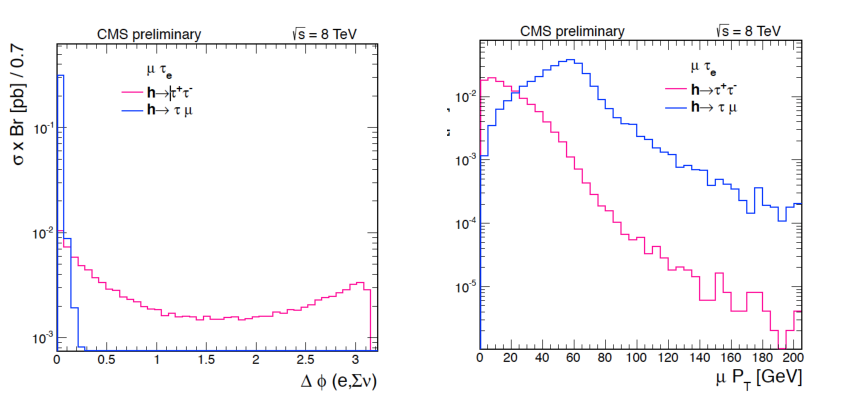
\includegraphics[width=0.8\textwidth,keepaspectratio]{plots_and_figures/chapter5/htt_v_lfv.pdf}
\caption{Illustration of the differences in $\pt^{\Pgm}$ and $\dphiemet$ spectrums in $\hmue$ and $\text{h} \to \Pgt_{\Pgm}\Pgt_{\Pe}$ processes.}
\label{fig:htt_v_lfv}
\end{center}
\end{figure*}

The most dominant backgrounds consists of \ztt events coming from Drell-Yan production and \ttb production. In \ztt events, one $\Pgt$ can decay to an $\Pe$ and the other to a $\Pgm$. This background peaks at lower values of $M_{col}$ than the signal events but there is significant overlap with the signal spectrum. In \ttb production, each of the top quarks can decay into a bottom and a $\PW$ with the $\PW$ bosons then decaying to a $\Pe$ and $\Pgm$. The other backgrounds are smaller and include (in no particular order) electroweak diboson production ($\PW\PW$, $\PW\PZ$ and $\PZ\PZ$), h boson decays allowed by the SM ($\PH \to \Pgt\Pgt,\PW\PW$), $\PW\gamma^{(*)}+\text{jets}$ ,single top production, \wjets events, $Z\to\ell\ell$ $(\ell = \Pe, \Pgm)+\text{jets}$ and QCD multijet backgrounds. These backgrounds are described in more detail, along with there estimation and validation techniques in section~\ref{bg_val}.        


\subsection{\hmue:Baseline selection and categorization}
\label{h125_presel_cat}
A baseline selection is defined first in order to ensure that we have clean and well-defined events faithful to the final state signature of the signal process. An isolated and well-identified $\Pgm$ is thus required to be present along with a well-identified and isolated $\Pe$ of opposite sign charge. They are required to be separated by $\Delta R > 0.3$. The identification criterion applied for $\Pgm$ and $\Pe$ have been described in sections~\ref{mu_recon} and~\ref{e_recon}. Isolation criterion, as measured by $I_\text{rel}$ (described in ~\ref{tau_recon}), are required to have values $I_\text{rel}^{\Pe} < 0.15$ and $I_\text{rel}^{\Pgm} < 0.1$. The $\pt$ of these candidates are required to be above minimal thresholds required by trigger, identification and isolation requirement. Both candidates are also required to be within the fiducial region of the detector. The $\Pgm$ is required to have $\pt^{\Pgm} > 26$\GeV and $|\eta^{\Pgm}|<2.4$.The $\Pe$ is required to have $\pt^{\Pe} > 10$\GeV and $|\eta^{\Pe}|<2.3$. Only events with two or fewer jets are considered. All jets considered must have $\pt>30$\GeV, $|\eta| < 2.4 $ and satisfy the loose identification criterion described in section~\ref{jet_recon}. Events with one or more jets arising from a b-quark (b-tagged jets) are vetoed. Cleaning events with b-tagged jets reduce some contribution from backgrounds which give rise to b-quarks such as \ttb and single top. Also, as described in~\ref{jet_recon}, any event with one or more jets within $\Delta R < 0.4$ of either lepton candidates is also rejected. Further, an event is rejected if it has additional $\Pgm$ or $\Pe$, or any $\Pgt_{had}$ candidates. All the above baseline selection requirements have been summarized in Table~\ref{tab:h125_base_sel}. All the events were required to pass isolated muon triggers with a $\pt$ threshold of 24 \GeV. The trigger selection has been described in detail in section~\ref{trigger}. The distributions of the \mcol and several other kinematic variables after the baseline selection just described, are shown in Figs.~\ref{fig:h125_presel1} and ~\ref{fig:h125_presel2}. These distributions act as the starting point for development of stricter kinematic selections looking at the different shapes of signal and backgrounds distributions for different variables.     


\begin{table*}[htpb]
 \begin{center}
 \caption{Baseline selection criteria for \hmue analysis.}
  \begin{tabular}{c|c|c} \hline
    Variable    &  $\Pgm$  & $\Pe$ \\ \hline
    $\pt $       & $>30$\GeV &  $>10$\GeV                                           \\
    $|\eta| $       & $<2.4 $ &  $<2.3$                                           \\
    $I_{\text{rel}}$  & $<0.15$ &  $<0.1$                                           \\
    \multicolumn{3}{c}{Cleaning requirements} \\\hline
    \multicolumn{3}{c}{ $\Delta R(\Pgm,\Pe) > 0.3$} \\ 
    \multicolumn{3}{c}{No additional $\Pgm$, $\Pe$ or $\Pgt_{had}$} \\
    \multicolumn{3}{c}{No b-tagged jets with $\pt>30$\GeV} \\
    \multicolumn{3}{c}{No jets with $\Delta R(\Pgm,jet)<0.4$ and $\pt>30$\GeV} \\
    \multicolumn{3}{c}{No jets with $\Delta R(\Pe,jet)<0.4$ and $\pt>30$\GeV }\\
    \hline
  \end{tabular}
  \label{tab:h125_base_sel}
  \end{center}
\end{table*}


\begin{figure*}[!htpb]\centering
 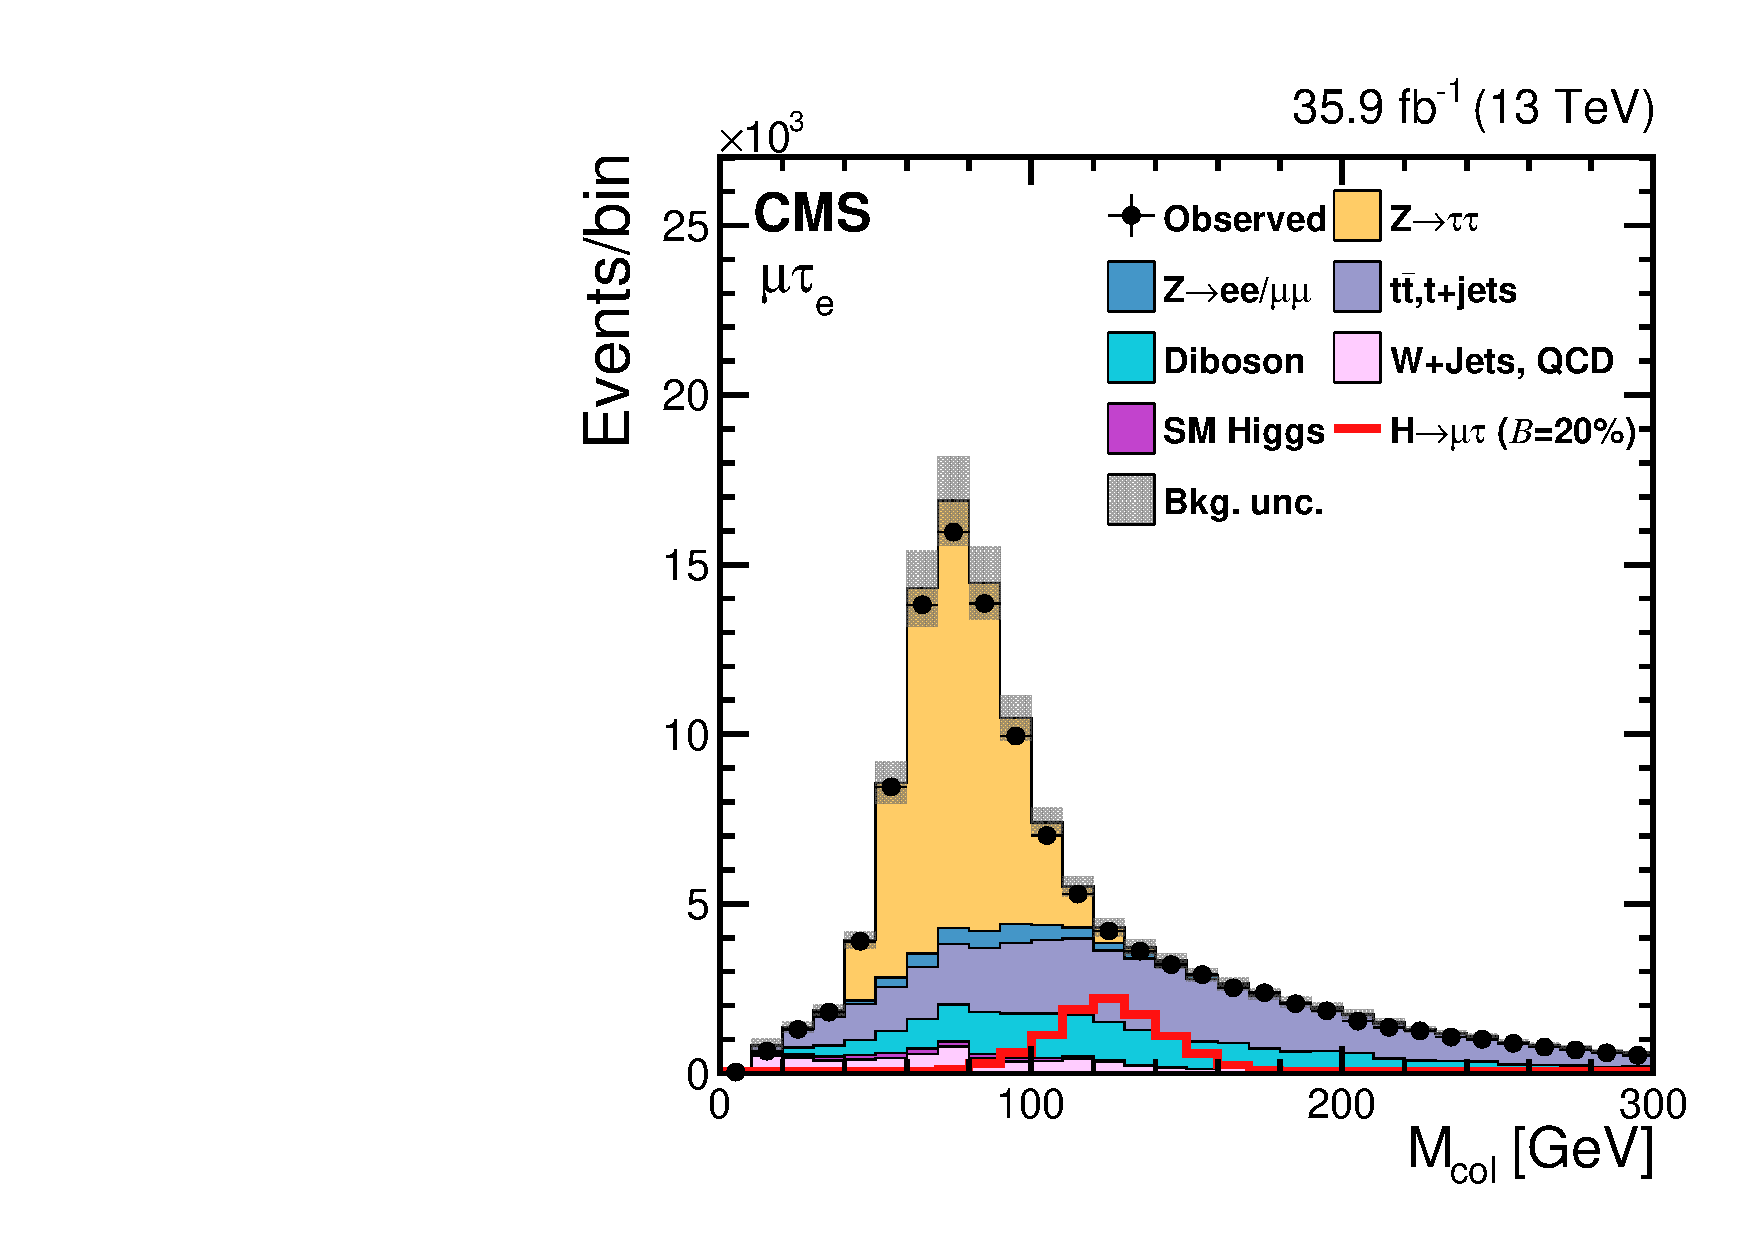
\includegraphics[width=0.49\textwidth]{plots_and_figures/chapter5/preselection/Figure_002-a.pdf}
 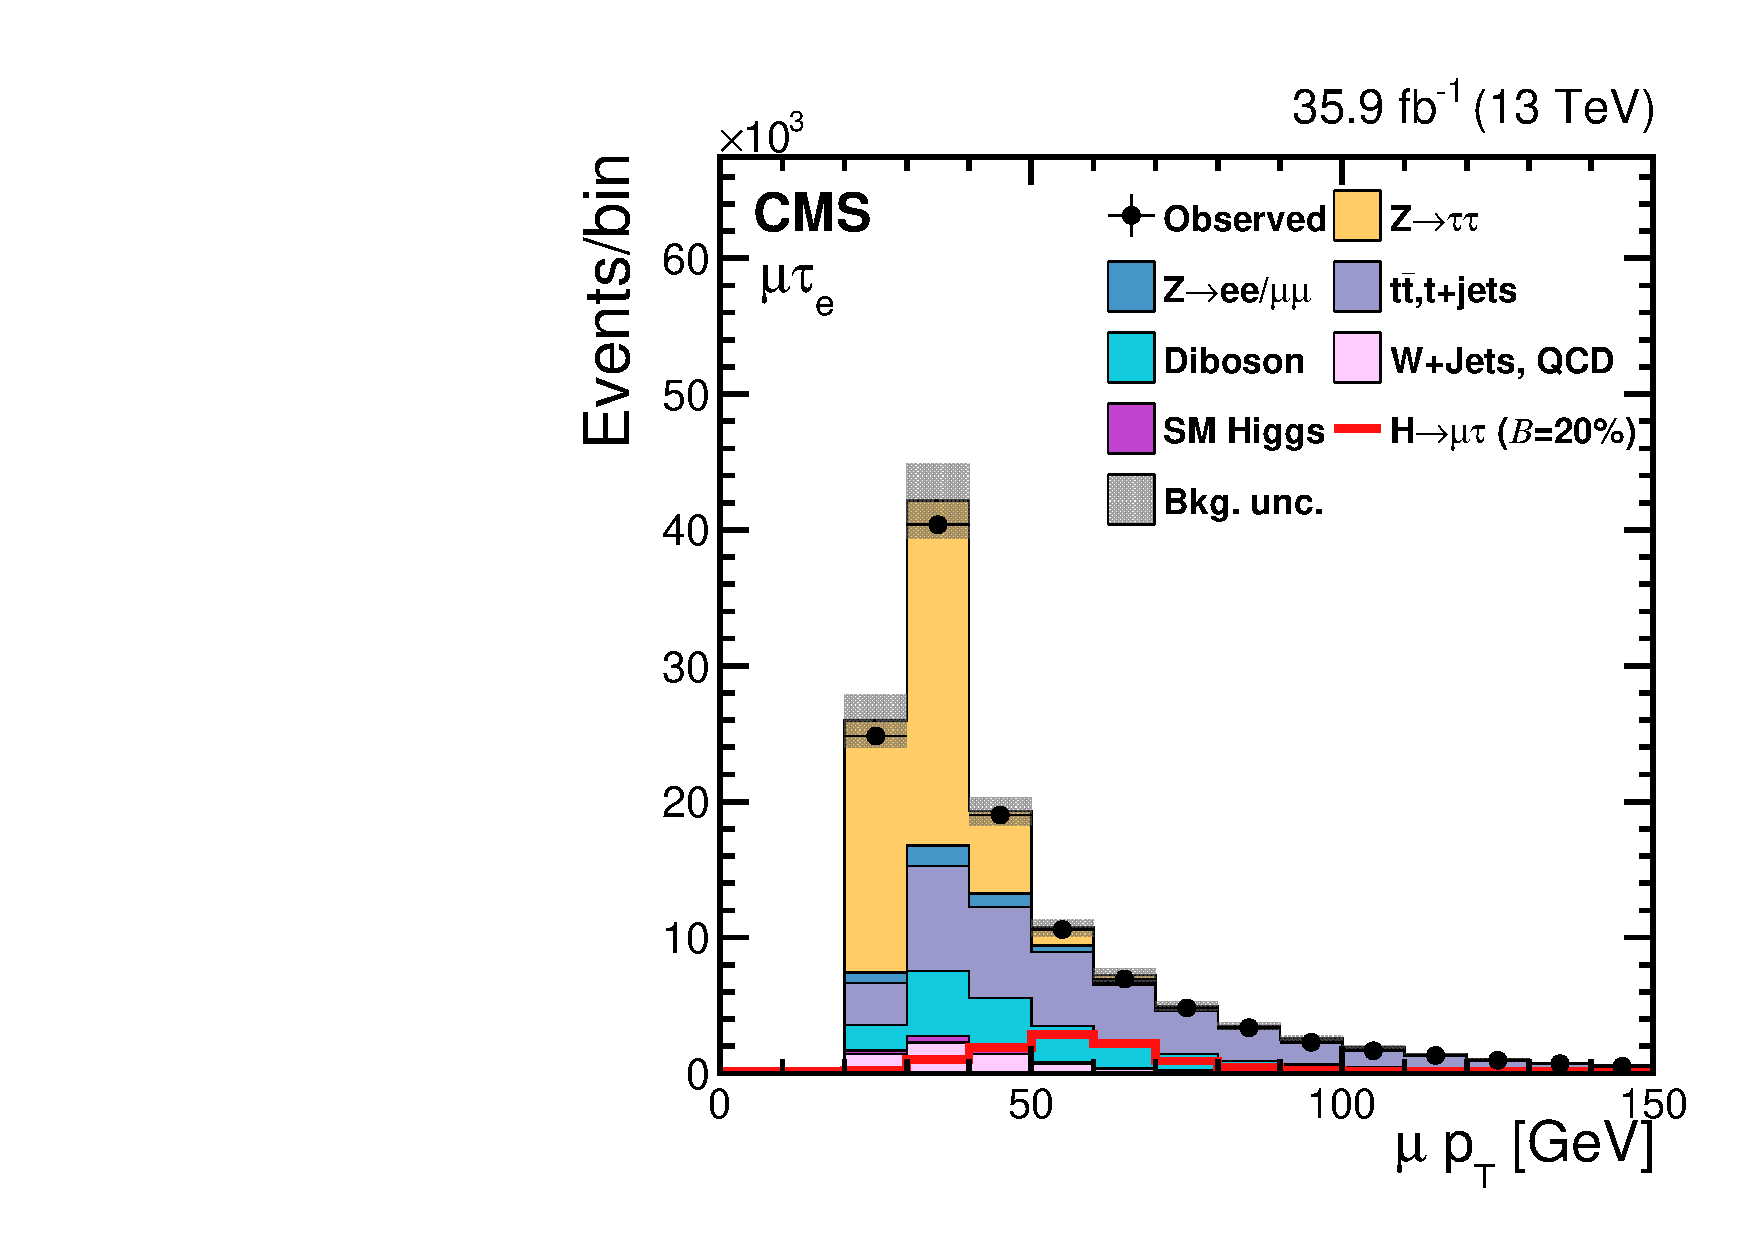
\includegraphics[width=0.49\textwidth]{plots_and_figures/chapter5/preselection/Figure_002-b.pdf} \\
 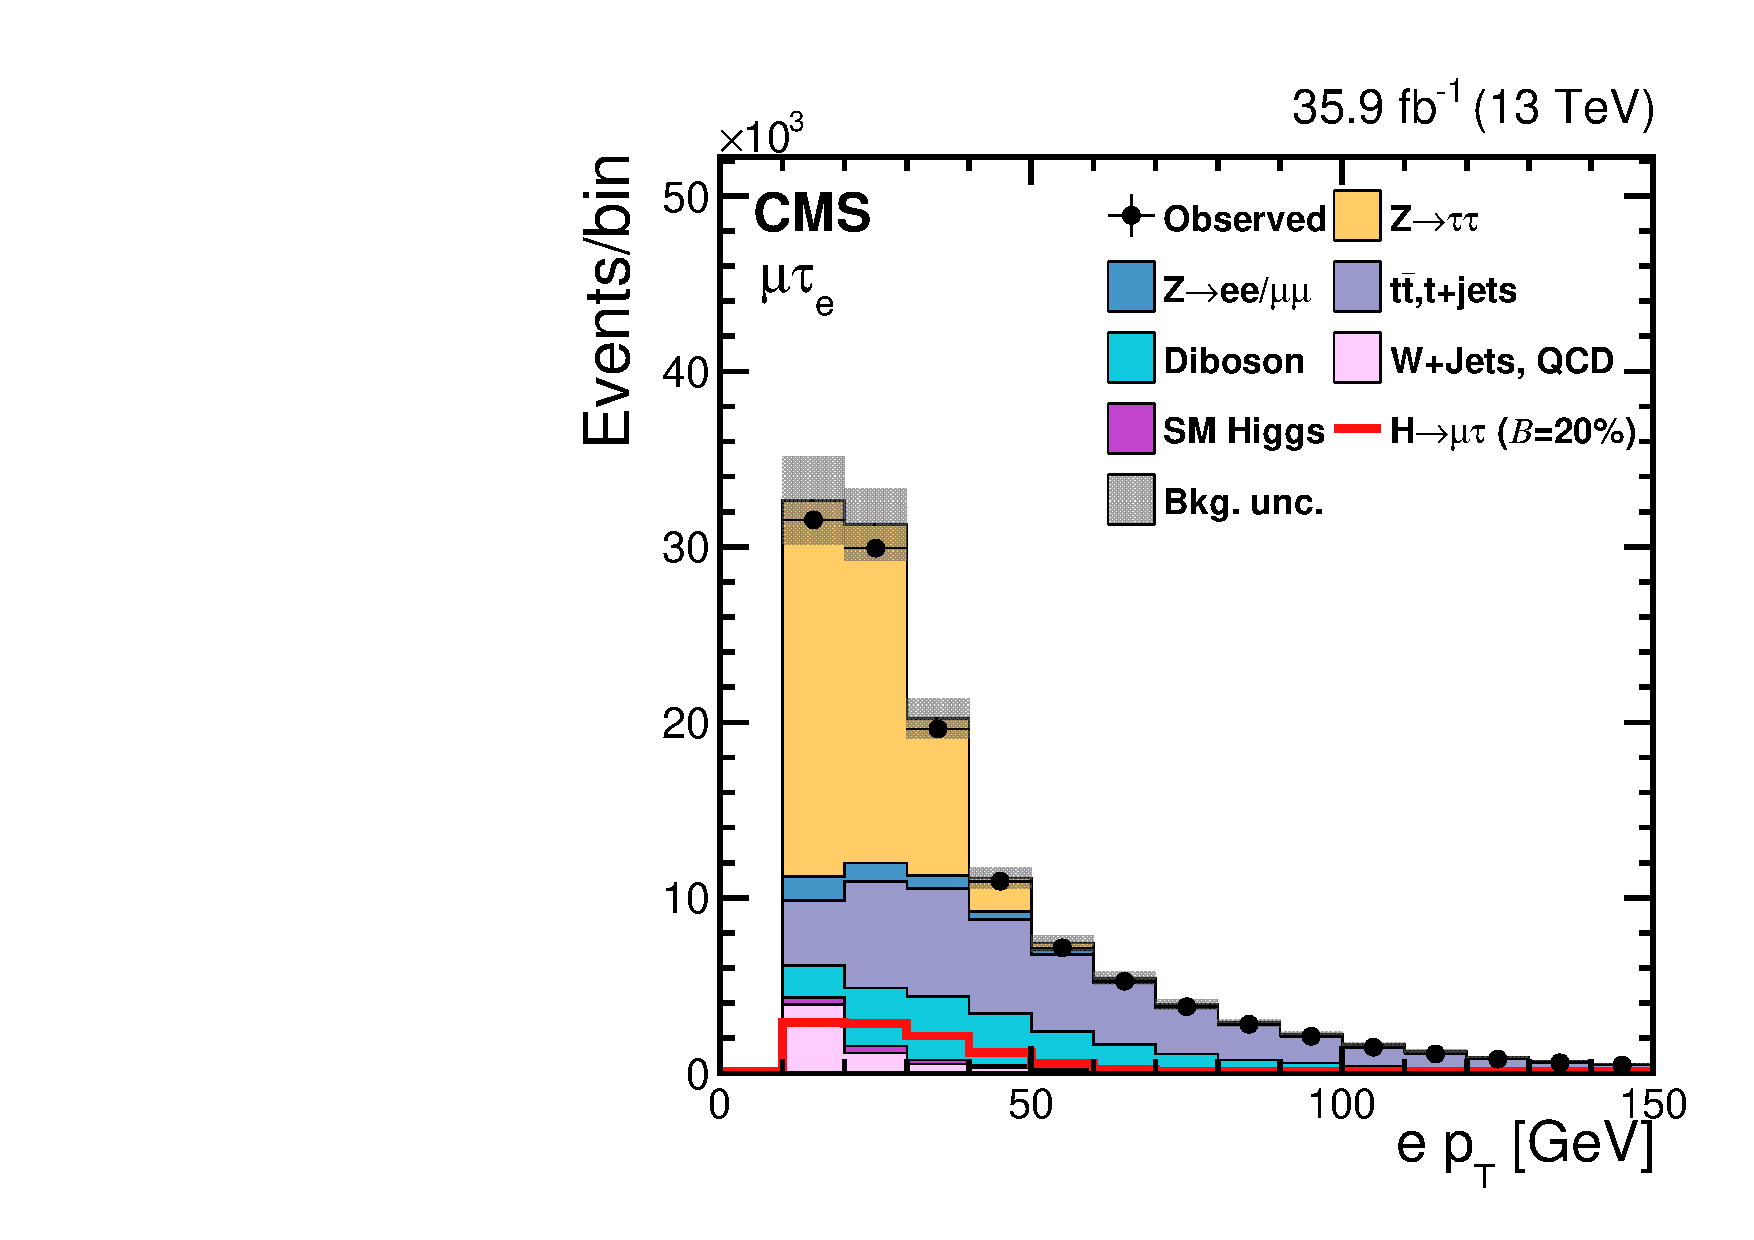
\includegraphics[width=0.49\textwidth]{plots_and_figures/chapter5/preselection/Figure_002-c.pdf}
 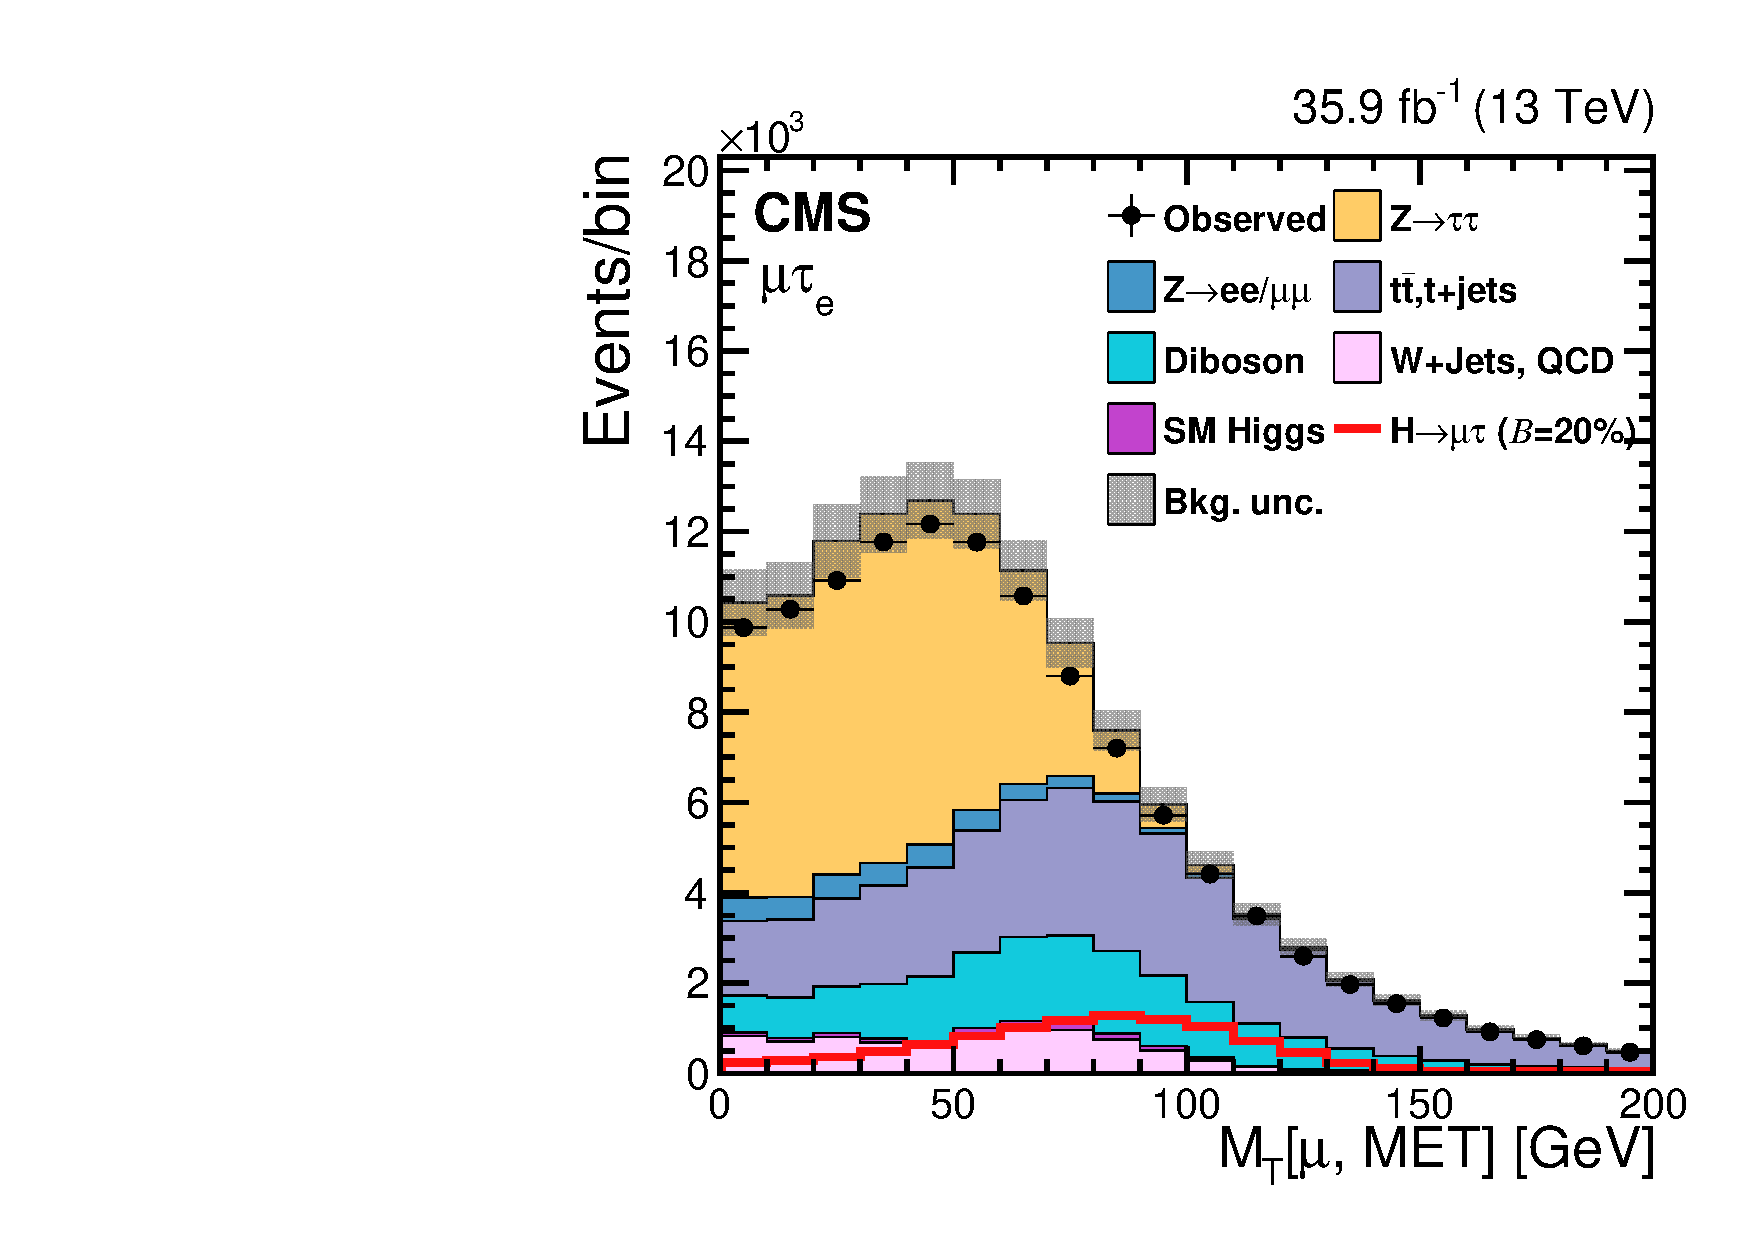
\includegraphics[width=0.49\textwidth]{plots_and_figures/chapter5/preselection/Figure_002-d.pdf} 
\caption{Distributions of kinematic variables after baseline selction for \hmue analysis (1).}
 \label{fig:h125_presel1}
\end{figure*}
\begin{figure*}[!htpb]\centering
 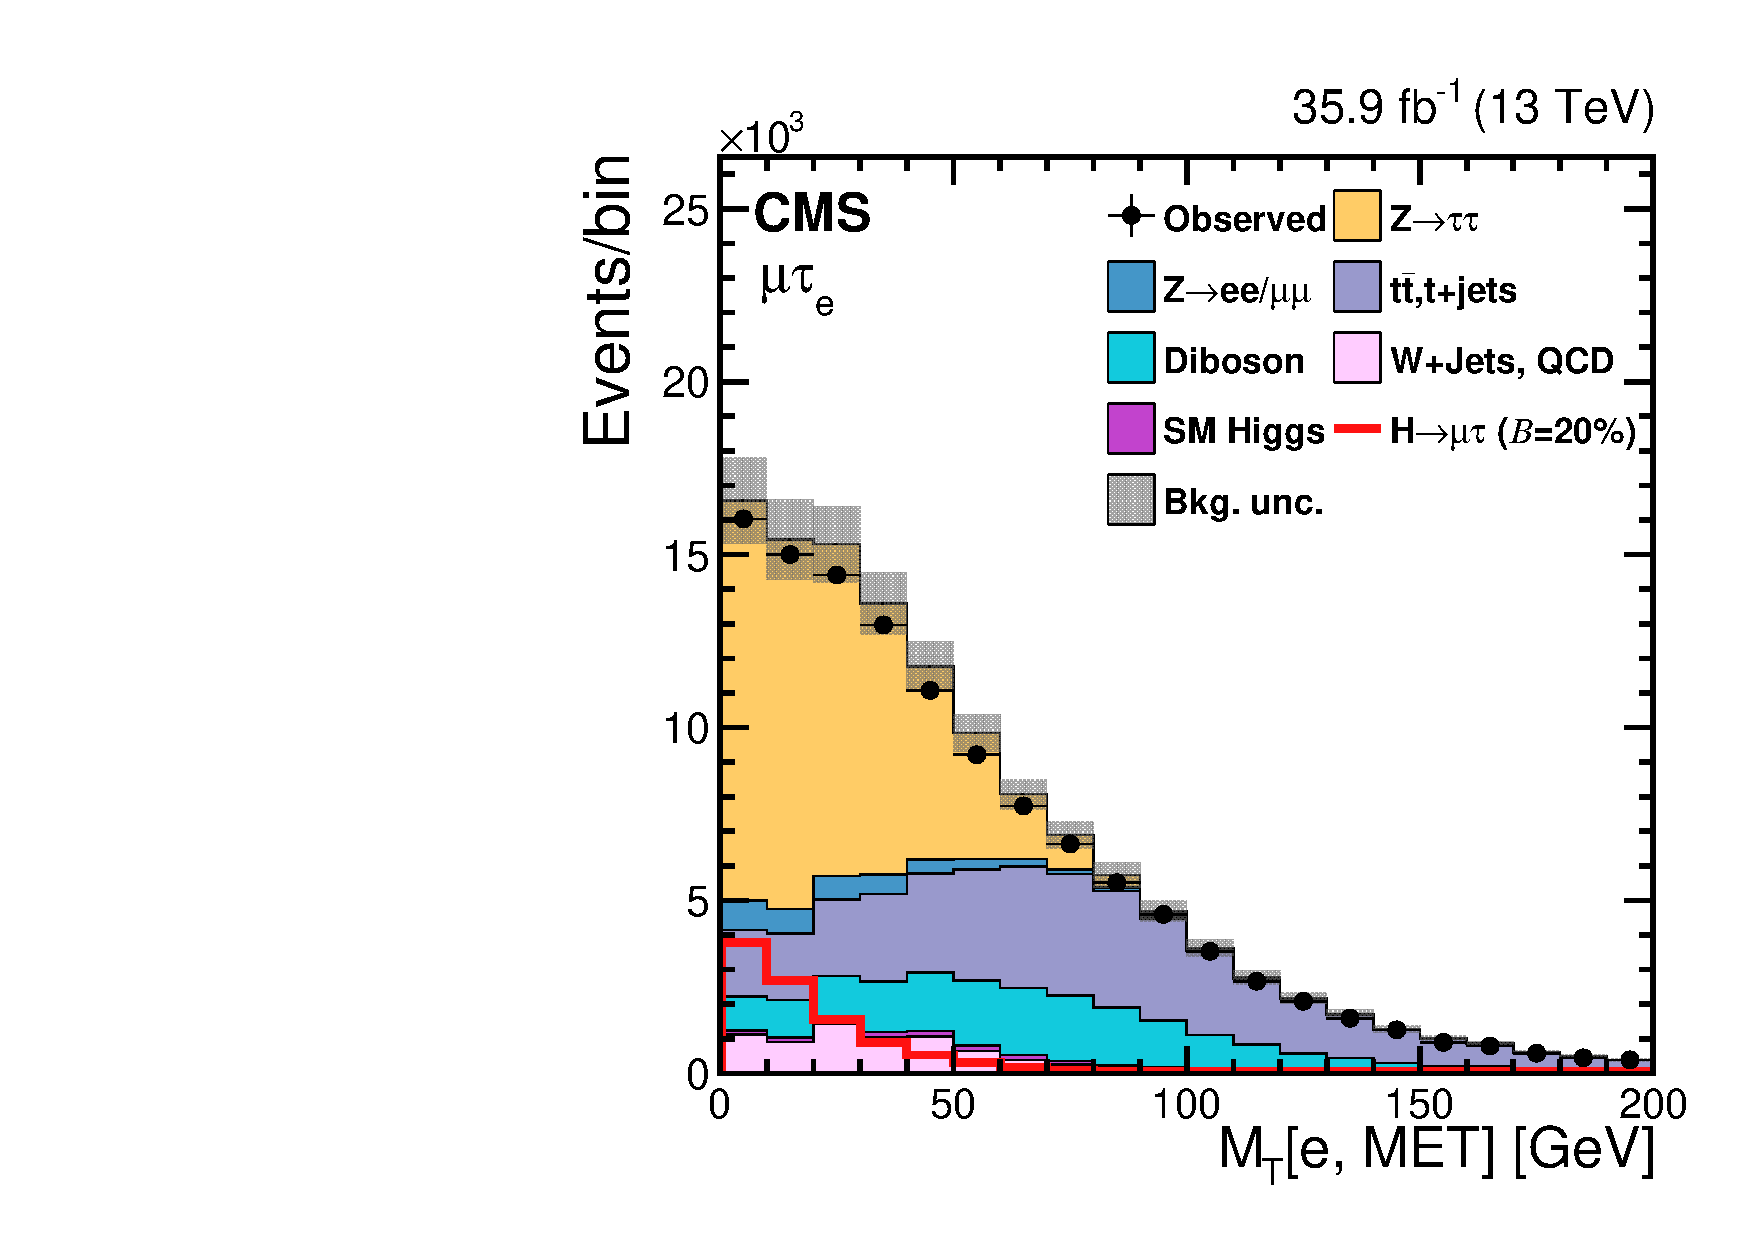
\includegraphics[width=0.49\textwidth]{plots_and_figures/chapter5/preselection/Figure_002-e.pdf}
 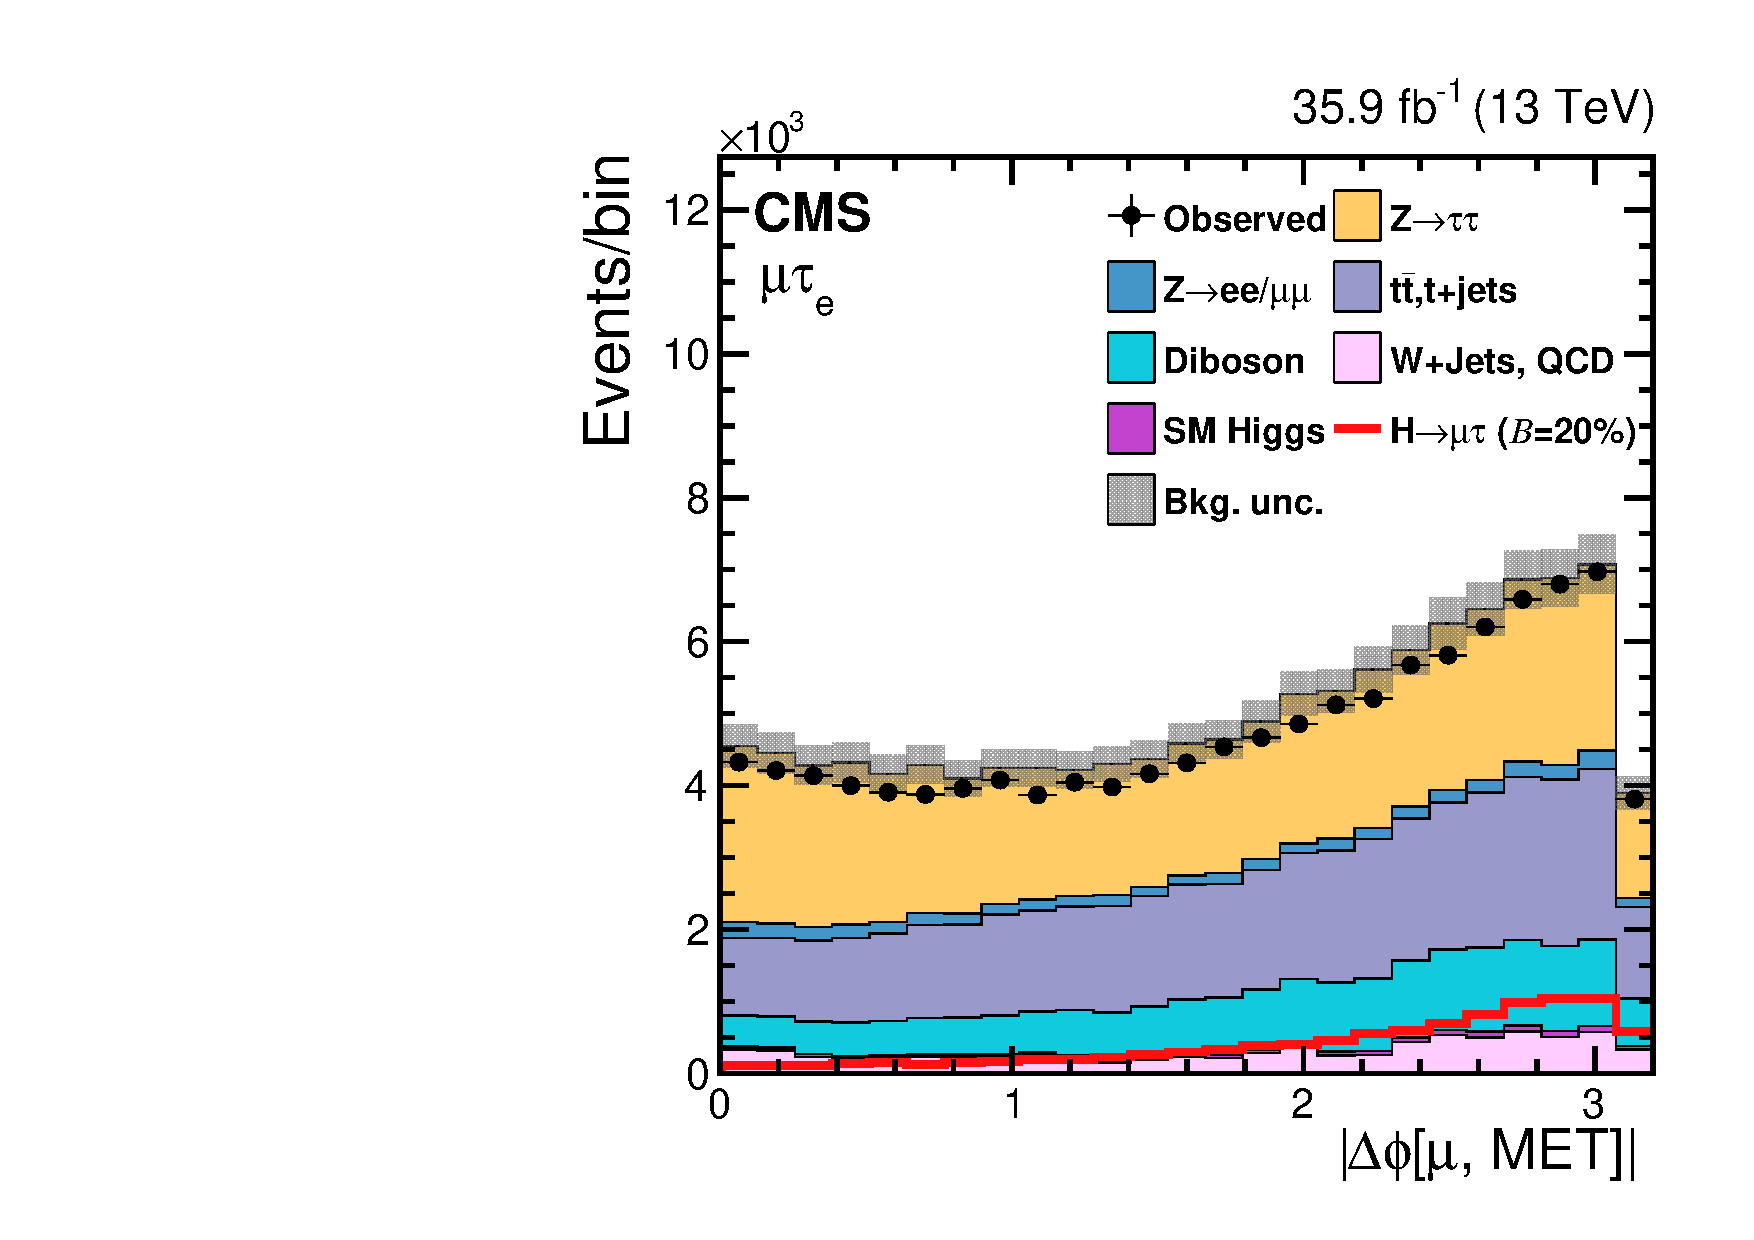
\includegraphics[width=0.49\textwidth]{plots_and_figures/chapter5/preselection/Figure_002-f.pdf} \\
 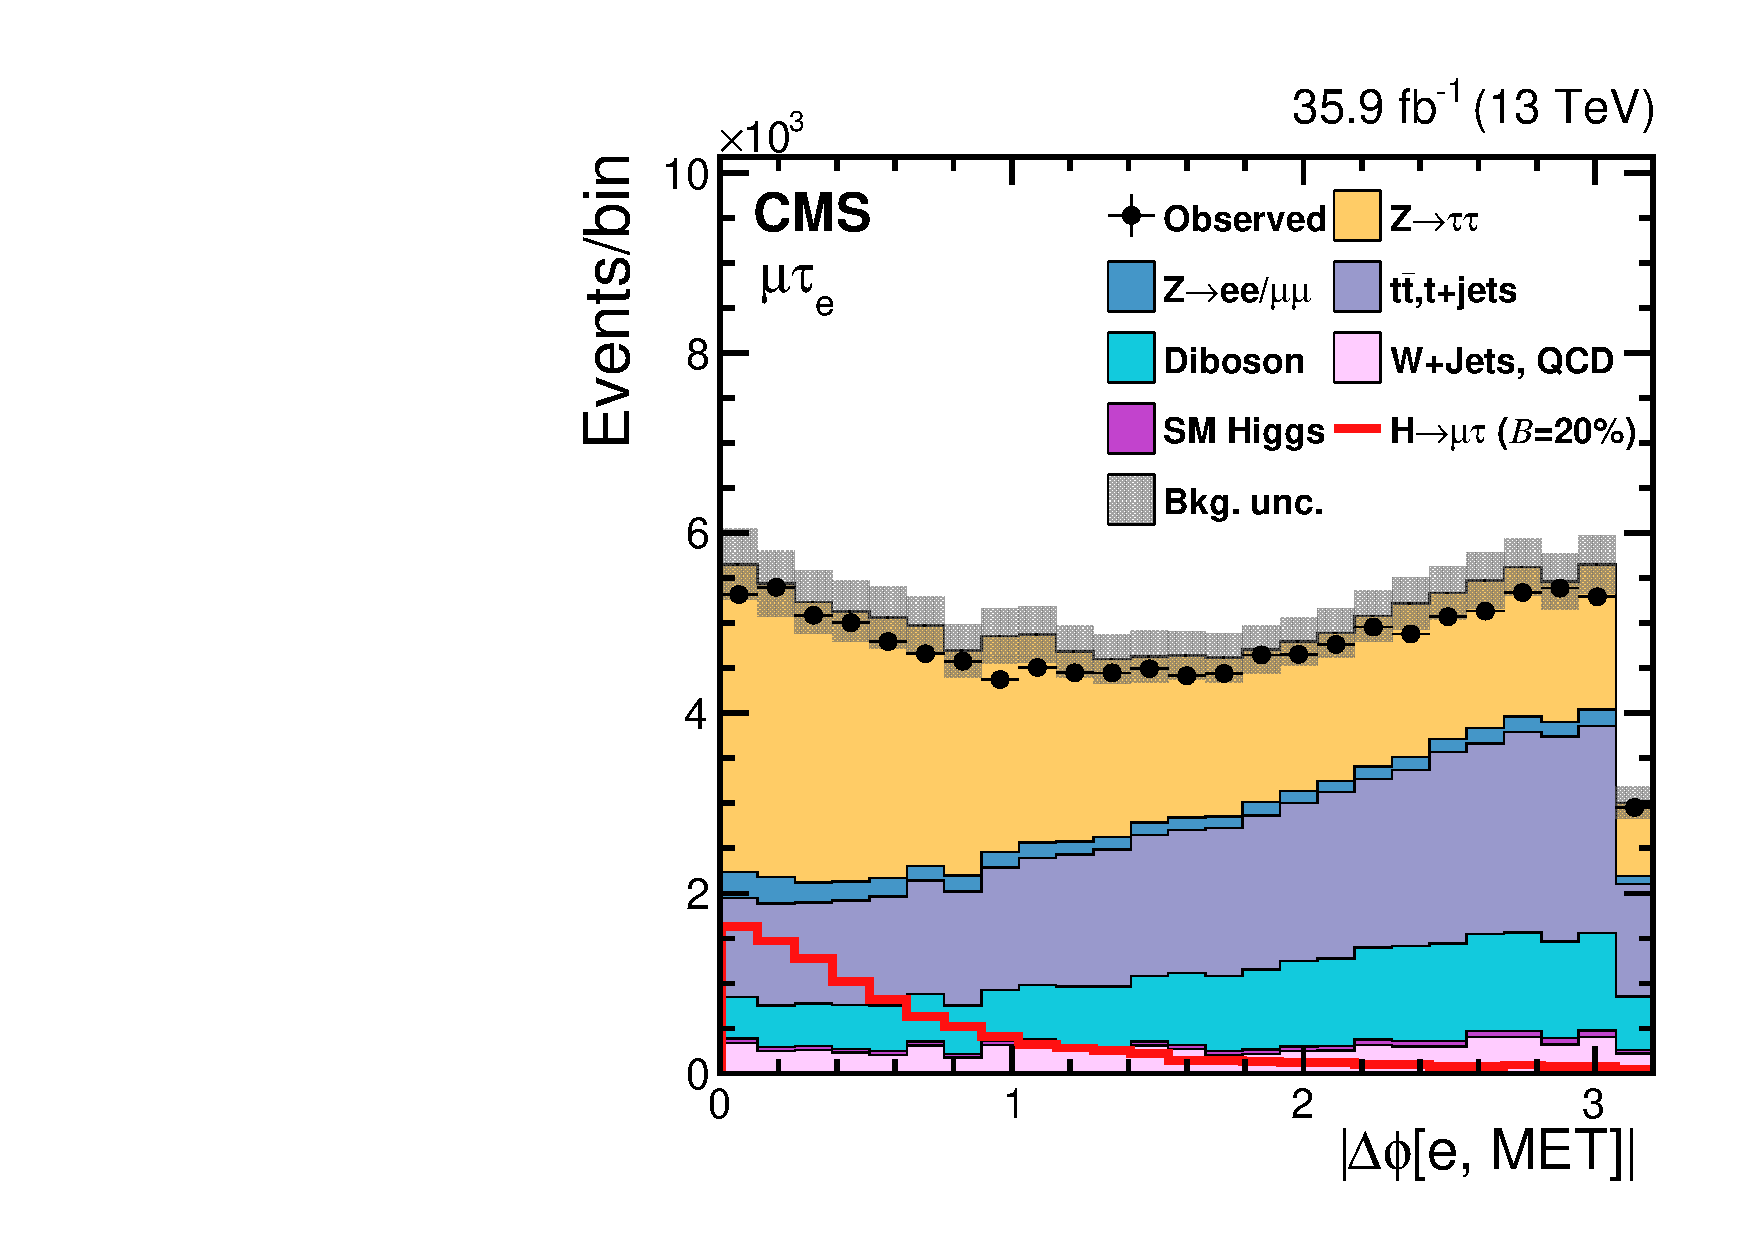
\includegraphics[width=0.49\textwidth]{plots_and_figures/chapter5/preselection/Figure_002-g.pdf}
 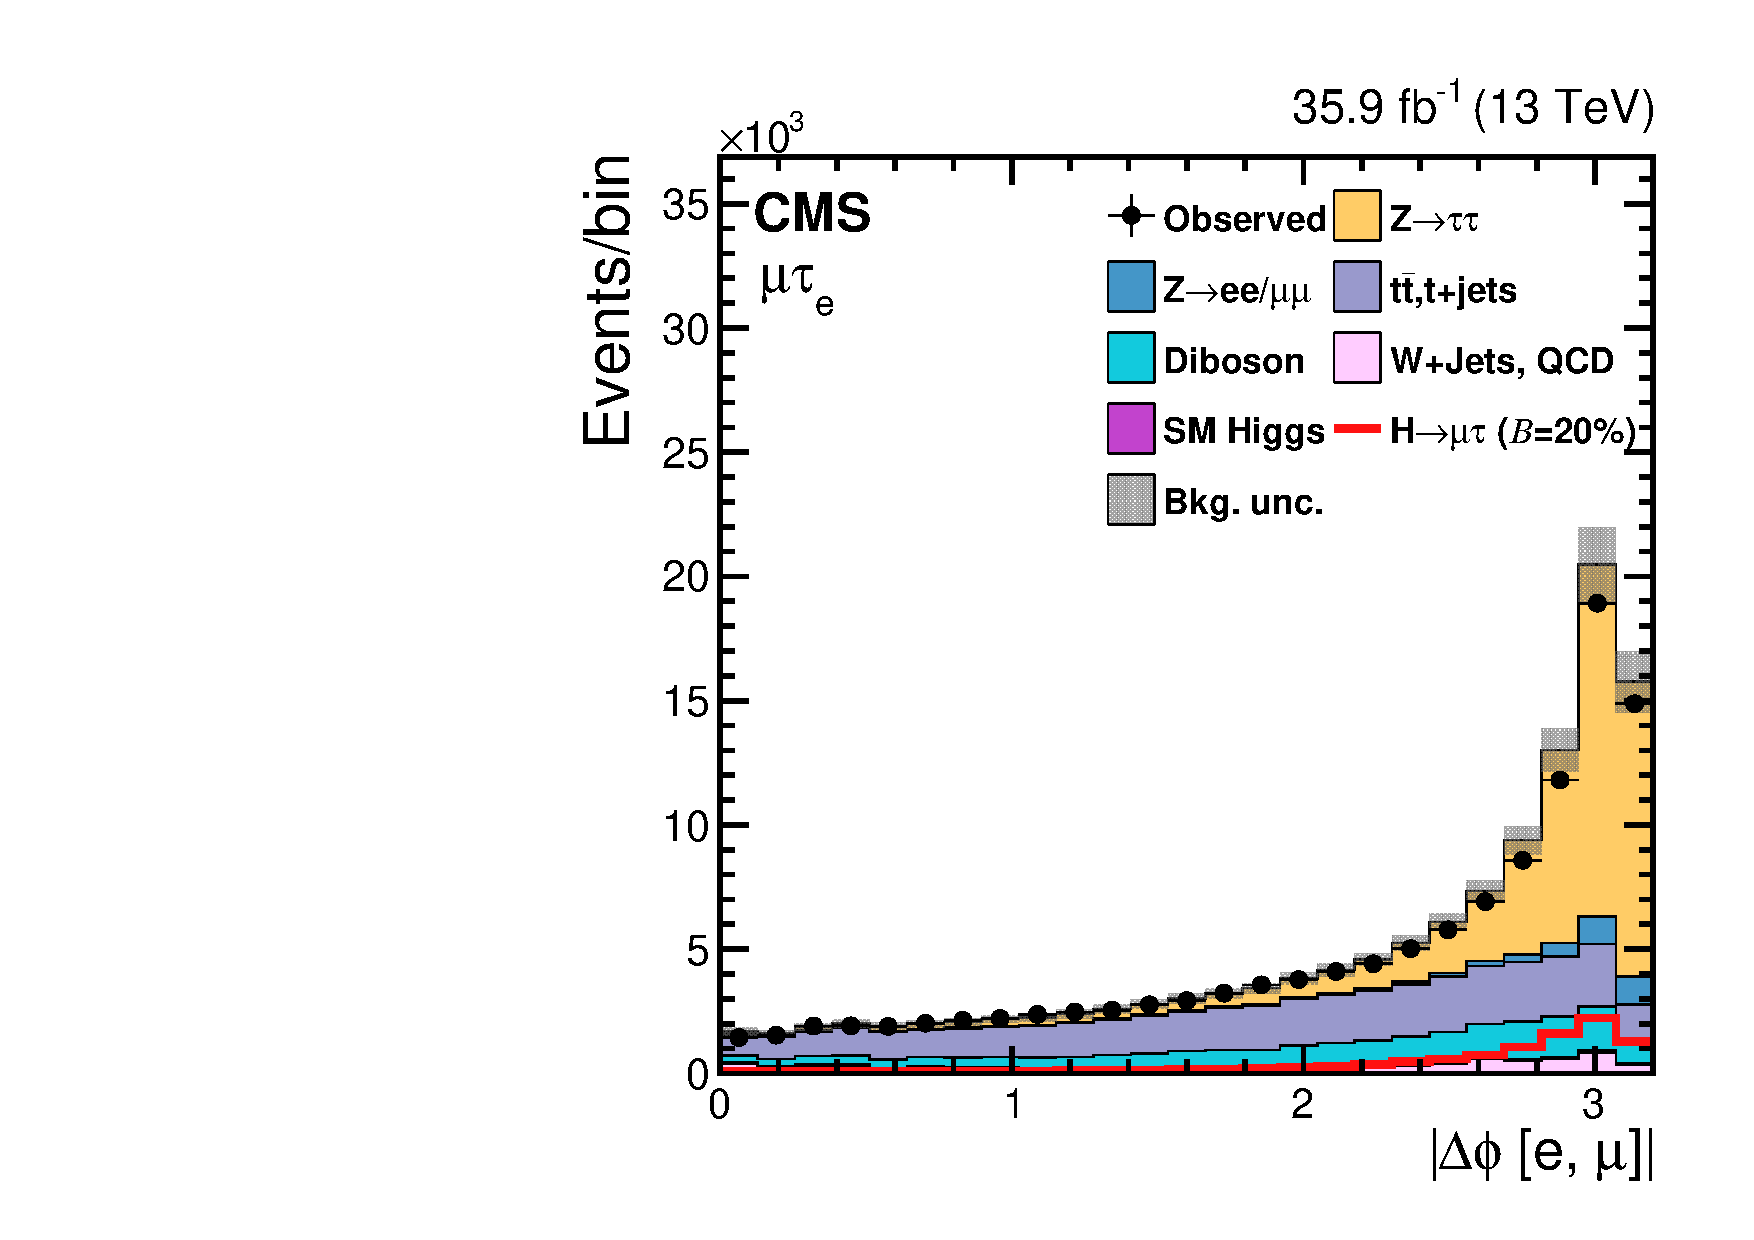
\includegraphics[width=0.49\textwidth]{plots_and_figures/chapter5/preselection/Figure_002-h.pdf}
\caption{Distributions of kinematic variables after baseline selction for \hmue analysis (2).}
 \label{fig:h125_presel2}
\end{figure*}

At this point the events are divided into several buckets, called categories. This is done on the basis of number of jets present in the event. In events with 2 jets the invariant mass of the di-jet system ($M_{jj}$) is also used for categorization. The topology of events containing different number of such jets can be different. For example, in events with one energetic jet the h produced can be boosted resulting in the azimuthal separation of the $\Pgm$ and $\Pe$ (that come from its decay) to be narrower than events with no jets. Each of this categories enchance the contribution of different h boson production mechanisms, and requiring different optimal selection criteria in each category  helps increase the sensitivity of the search. The categories in order of decreasing number of signal events are:
\begin{itemize}%[itemsep=5pt]
\item \textbf{0-jet category}: These are events that do not have any jet. This category enhances the gluon-gluon fusion (GGF) contribution.
\item \textbf{1-jet category}: Events that have 1 jet are put in this category. This category enhances the GGF production with initial state radiation (ISR). Some VBF events where one jet has escaped detection can also enter this category.
\item \textbf {2-jet GGF category}: This category contains events that have 2 jets with the additional requirement that $M_{jj}<550$\GeV. The dominant contribution comes from GGF production in association with two jets.
\item \textbf{2-jet VBF category}: This category contains events that have 2 jets with the additional requirement that $M_{jj}\geq 550$\GeV. The dominant contribution comes from VBF production which is characterized by presence of two jets with high dijet mass.  
\end{itemize}

\subsection{\hmue: \mcol fit selection}
\label{h125_cb_sel}
In the \mcol fit method, the selection is performed by placing kinematic cuts on several variables to enhance the signal-to-background ratio. There are several variables considered for this and they include: the azimuthal separation ($\Delta\phi$) between $\Pgm$ and $\Pe$, between $\Pe$ and $\ptvecmiss$, between $\Pgm$ and $\ptvecmiss$, denoted respectively by $\dphiemu$, $\dphiemet$, $\dphimumet$ , and the transverse mass between $\Pgm$ and $\ptvecmiss$, between $\Pe$ and $\ptvecmiss$, devnoted respectively by $M_T(\Pgm)$ and $M_T(\Pe)$. The \hmue decay being a 2-body decay, the $\Pgm$ and $\Pe$ are expected to be well separated in the azimuthal plane. Therefore, selecting events with a $\dphiemu$ larger than a threshold can help reject background events while keeping the signal that is peaked at high $\dphiemu$ values. This can be seen from Fig~\ref{fig:h125_presel2} (bottom right). Both neutrinos in the signal process come from the decay of the same $\Pgt$. These neutrinos form the $\ptvecmiss$. As mentioned earlier, the $\Pgt$ being much lighter than the h, it is highly boosted and its decay products i.e. $\Pe$ and the $\ptvecmiss$ are expected to be close to each other in the azimuthal direction. Thus $\dphiemet$ is expected to peak at values close to zero for signal events, as seen in Fig~\ref{fig:h125_presel2} (bottom left). Given that all backgrounds have relatively flat shape for this variable  throughout the $\Delta\phi$ range, requiring $\dphiemet$ to be lower than a threshold works as a strong rejection criterion against the backgrounds. Following a similar line of reasoning, the $\Pgm$ is expected to be well separated from the $\ptvecmiss$ resulting in $\dphimumet$ for signal events to peak at high values, as seen in Fig~\ref{fig:h125_presel2} (top right). Further, as the $M_T(\ell)$ (defined in section ~\ref{col_mass}) contains negative of the cosine of $\Delta\phi(\ell, \ptvecmiss)$ term, it is expected to be peak at values similar to $\Delta\phi(\ell, \ptvecmiss)$. This can be seen from Fig ~\ref{fig:h125_presel2} (top left) and Fig~\ref{fig:h125_presel2} (bottom right) which show signal events for $M_T(\Pgm)$ and $M_T(\Pe)$ peak at relatively higher and lower values than most backgrounds respectively. In particular, requiring $M_T(\Pgm)$ to be larger than a threshold can help reject a lot of \ztt events which is the most dominant background in the 0-jet category. All the above variables have some amount of correlation with one another (see the correlation matrix shown in Fig.~\ref{fig:bdt_corr_mat}. The optimization procedure used to arrive at the most optimal set of kinematic thresholds for these variables is described in detail in the next paragrhaph. The thresholds on the $\pt$ of the $\Pgm$ and $\Pe$ have not been made stricter to avoid biasing the selection toward energetic leptons that sculpt the background $\mcol$ distribution to mimic the signal peak. This effect could potentially reduce the shape discrimination power of the signal extraction procedure. Only in the 0-jet category category the requirement on $\pt$ of the $\Pgm$ is made marginally stricter by requiring  $\pt^{\Pgm} > 30$\GeV. All other lepton $\pt$ requirements are allowed to remain the same as baseline selection and are not included in the optimization procedure.   

The aim of the optimization procedure is to maximize the sensitivity of the analysis. In other words, we want to select a set of thresholds which increases a quantity such as the $\frac{S}{\sqrt{S+B}}$ ratio where S and B are the number of estimated signal and background events respectively. It is also necessary to ensure alongwith, that the entire spectrum of distribution of the discriminant variable (that is used int the final max-likelihood fit to extract results) is well-populated, escpecially in the region where the signal is expected to appear. A bad fit can potentially degrade the sensitivity of the analysis. Taking both of the above points into consideration, the thresholds have been optimized to obtain the most stringent (lowest) possible expected limits. The definition and procedure of extacting the expected limit is given in section~\ref{exp_limits}). To do the optimization of the kinematic thresholds, we start by requiring the baseline selection. Then for a variable in consideration,e.g.- $\dphiemet$, we look at the expected limit while making the threshold progressively stricter until we reach a point where making the threshold any stricter degrades (increases) the expected limit. We repeat this procedure for all variables and note the stringent expected limit for each (by tightening thresholds of only that variable). This concludes one round of the optimization. For the next round we start by requiring the baseline selection. In addition we require that the variable that achieved the best possible expected limit among all variables in the last round satisfy its corresponding threshold. Lets call this variable variable1. We now repeat the same procedure as the last round for all but variable1. Say the variable that gave us the best possible expected limit this round is variable2. For the start of the following round variable2 is is required to satisfy its corresponding threshold. Then all the other variables (including variables that were had chosen thresholds in earlier rounds such as variable1 here) are made to go through the same procedure. This is done because the optimum value of threshold for variables chosen earlier might shift as new variables are chosen. This process is continued until the expected limit becomes no further stringent in sucessive rounds. This optimization was done separately for each of the four categories. The final set of thresholds arrived at in this way for the \hmue \mcol fit analysis are listed in Table.~\ref{tab:h125_sel_cuts}. This method of choosing the optimal set of thresholds is sometimes called the n-1 procedure, and the idea is conceptually similar to forward/backward selection methods used in statistical learning to build optimal models.             


\begin{table}[htpb]
 \begin{center}
 \caption{Final selection criteria for \hmue \mcol fit analysis.}
  \begin{tabular}{c|c|c|c|c} \hline
    Category     &  0-jet    & 1-jet & 2-jet GGF & 2-jet \\ \hline
    $\pt^{\Pgm}$ & $>30$\GeV &  --   & --        & --     \\
    $M_T(\Pgm)$  & $>60$\GeV & $>40$\GeV & $>15$\GeV & $>15$\GeV \\
    $\dphiemet$  & $<0.7$ & $<0.5$ & $<0.3$ & $<0.3$ \\
    $\dphiemu$   & $>2.5$ & $>2.0$ & -- & -- \\
    
    \hline
  \end{tabular}
  \label{tab:h125_sel_cuts}
  \end{center}
\end{table}
\subsection{\hmue: BDT method selction}
\label{h125_bdt_Sel}
In the BDT method, a boosted decision trees (BDT) classifier is used to discriminate signal events from background events. A decision tree is a classifier which works by building a tree structure based on binary splits (as shown in Fig.~\ref{fig:dec_tree}). Starting from the root node of the tree (which contains all the events which we want to classify), a sequence of binary splits is made using input variables provided to the classifier. At each split, the variable which provides best purity of split or equivalently, in our case the best separation of signal and background events, is used. The same variable can thus be used for splitting several nodes and the splitting is continued until a desired some stopping criterion such as depth of the tree, purity of leaf nodes , minimum number of events in a leaf node etc. is reached. All events end up in one of the leaf nodes. If an event ends up in a leaf node in which signal events form the majority fraction, it is classified as a signal event. Otherwise, it is classified as a background event. Boosting is a class of ensemble machine learning techniques which help in enhancing performance of weak classifiers by sequentially building classifiers using reweighted (boosted) versions of the training data and then taking a weighted majority vote of the sequence of classifiers thus produced. Boosting also stabilizes the response of the classifiers with respect to fluctuations in the training data. In other words it helps avoid overfitting to the training data. When the boosting technique is a applied to produce an ensemble of decision trees, the resulting ensemble of classifiers is called a Boosted Decision Trees classifier.

%A detailed overview of how decision trees and boosting works, and the chosen value of parameters used in training the BDTs for this analysis is given in appendix~\ref{chap_BDT}.

\begin{figure*}
\begin{center}
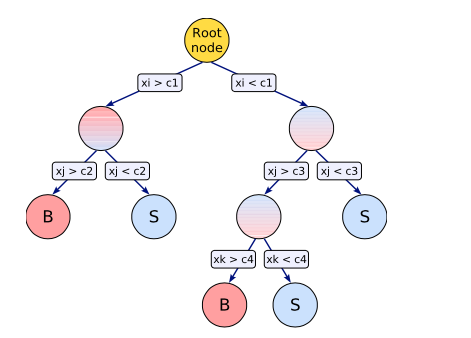
\includegraphics[width=0.8\textwidth,keepaspectratio]{plots_and_figures/chapter5/decision_tree.png}
\caption{Illustration of decision tree.~\cite{tmva_manual}}
\label{fig:dec_tree}
\end{center}
\end{figure*}


The BDT is trained using events that satisfy the baseline selection criteria. Simulated GGF and VBF events weighted by their cross-section are used as signal events for training. For background, a mixture of \ttb and Drell-Yan events are used, also weighted by their respective cross-sections. The \ttb and Drell-Yan backgrounds are the most dominant backgrounds. The Drell-Yan background is the most dominant background in 0-jet and 1-jet category, while the \ttb background is the most dominant in both 2-jet categories. It also has many kinematic characteristics in common with diboson and single-top bankgrounds. A suite of input variables is used in training of the BDT. They are as follows:
\begin{itemize}[itemsep=1pt]
\item Transverse mass between the $\Pgm$ and $\ptvecmiss$: $M_T(\Pgm)$.
\item Transverse mass between the $\Pe$ and $\ptvecmiss$: $M_T(\Pe)$. 
\item Azimuthal angle between the $\Pe$ and $\Pgm$: $\dphiemu$. 
\item Azimuthal angle between the $\Pe$ and $\ptvecmiss$: $\dphiemet$.
\item Azimuthal angle between the $\Pgm$ and $\ptvecmiss$: $\dphimumet$. 
\item Collinear mass: \mcol.
\item Muon \pt: $\pt^{\Pgm}$. 
\item Electron \pt: $\pt^{\Pe}$.
\end{itemize}
The distributions of these variables normalized to the total number of events in the input sample to the BDT is shown in Fig.~\ref{fig:bdt_inp_var}. The correlations between these variables in signal and background events are shown in Fig.~\ref{fig:bdt_corr_mat}.
\begin{figure*}
\begin{center}
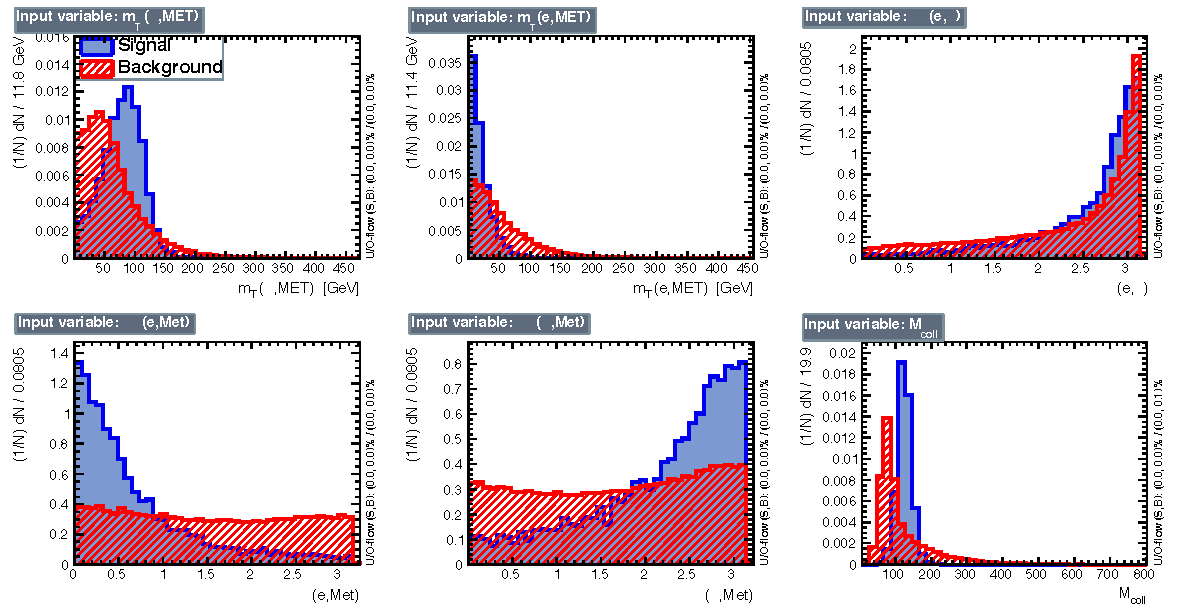
\includegraphics[width=0.9\textwidth]{plots_and_figures/chapter5/variables_id_c1.pdf}\\

\includegraphics[width=0.8\textwidth]{plots_and_figures/chapter5/variables_id_c2.png}\\
\end{center}
\caption{ Normalized distributions of the input variables for BDT method. The signal (blue) is composed of a weighted mixture of GGF and VBF events, whereas the background (red) is made of $t\bar{t}$ and Drell-Yan events. All events were required to satisfy the baseline selection criteria.}
\label{fig:bdt_inp_var}
\end{figure*}

\begin{figure*}[htpb]
\begin{center}
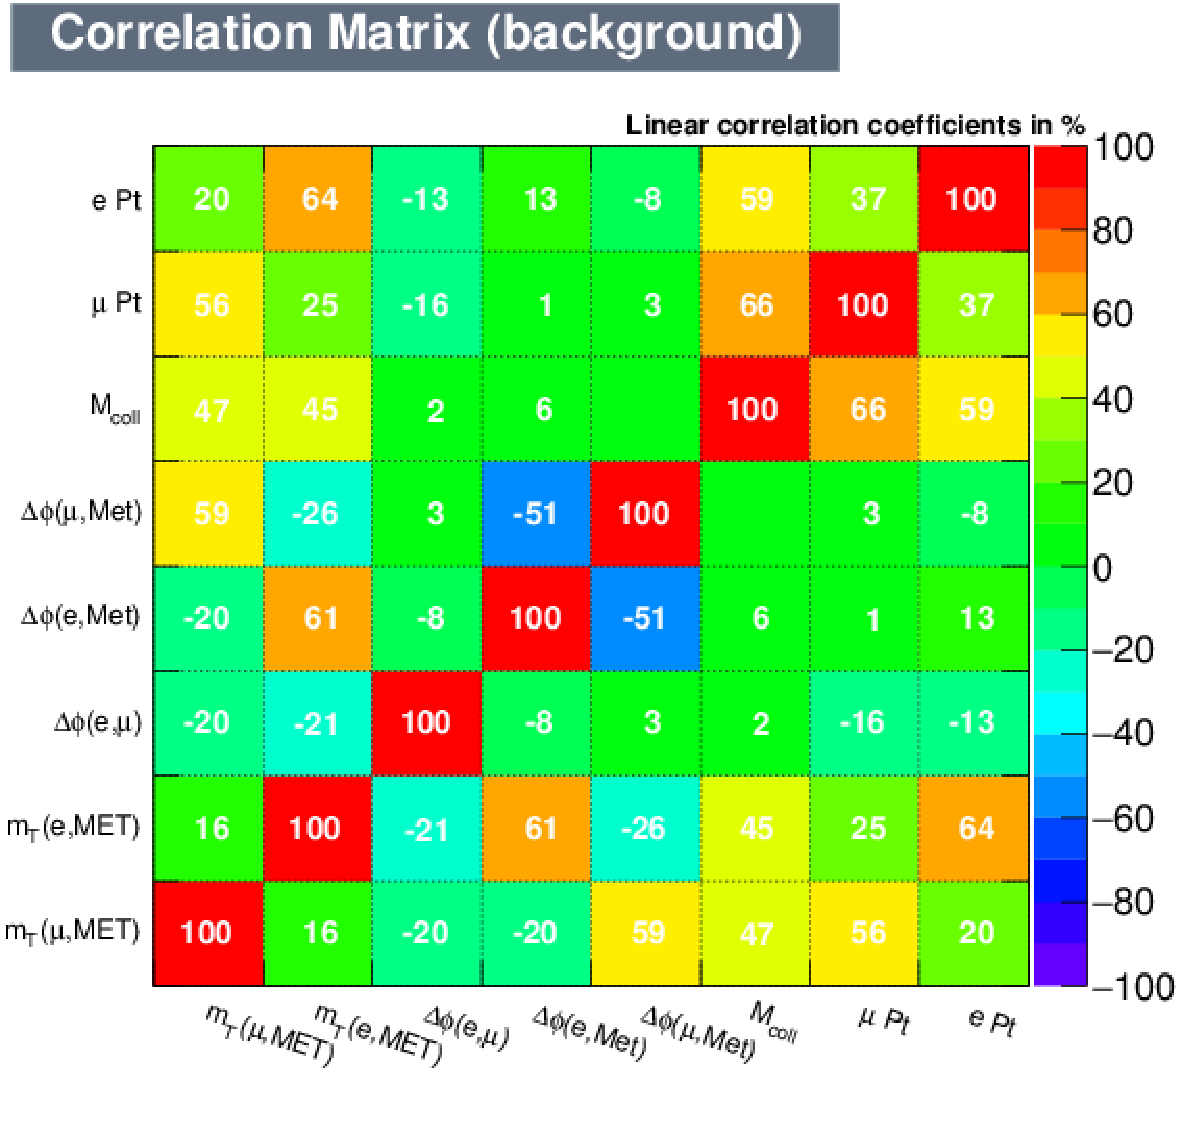
\includegraphics[width=0.48\textwidth]{plots_and_figures/chapter5/CorrelationMatrixB.pdf}
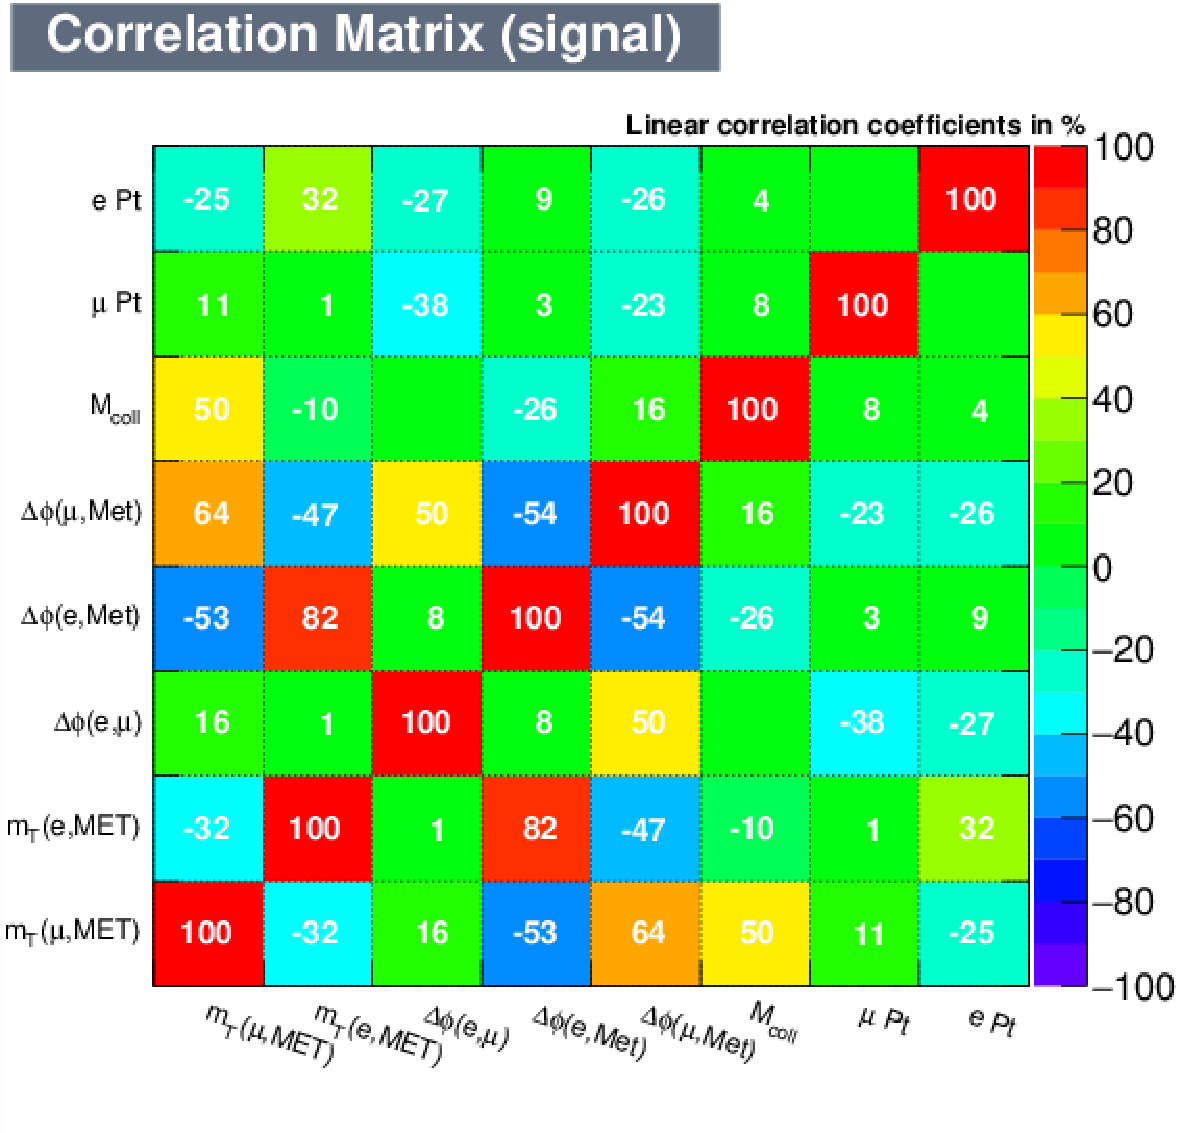
\includegraphics[width=0.48\textwidth]{plots_and_figures/chapter5/CorrelationMatrixS.pdf}\\
\end{center}
\caption{ Correlations between input variables for signal events (right) and background events (left).}
\label{fig:bdt_corr_mat}
\end{figure*}

The training was done with a 800 decision tree ensemble, each tree having a maximum depth of 4. The gini-index criterion was used for splitting the data at each node. Further, AdaBoost (adaptive bossting) method was used for boosting. A training to testing split of 70:30 split was used. Fig.~\ref{fig:BDT_response} shows the distribution of the BDT response for training and testing samples. The training and testing distributions for both signal and background events match well, suggesting that there is no overtraining. The distribution of BDT response is used in max-likelihood fit to extract results, as discussed in section~\ref{sig_ext}.  

\begin{figure*}[htpb]
\begin{center}
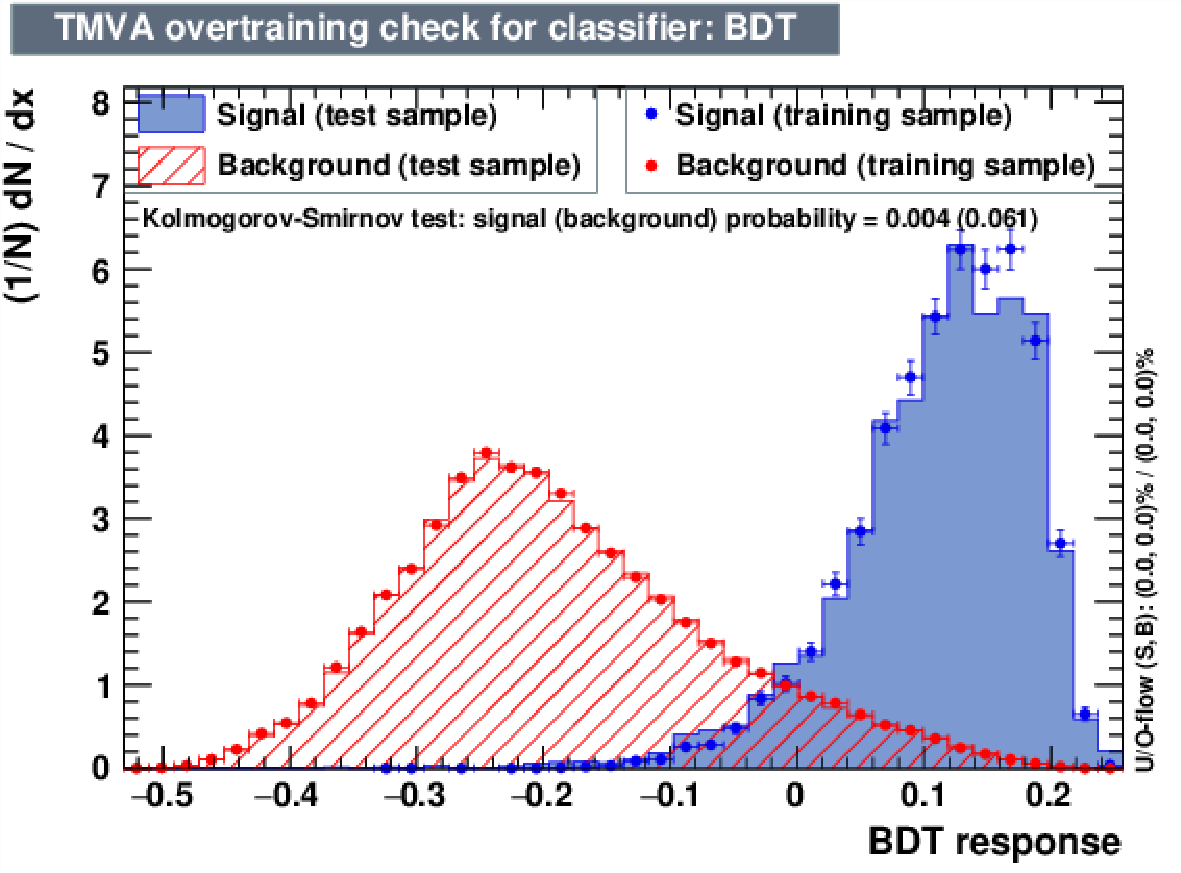
\includegraphics[width=0.48\textwidth]{plots_and_figures/chapter5/overtrain_BDT.pdf}
\end{center}
\caption{Distribution of BDT response for training (dots) and test(fill) distributions for both signal(blue) and background(red) events.}
\label{fig:BDT_response}
\end{figure*}

\section{ Heavy higgs:\Hmue analysis}
\subsection{\Hmue: Final state signature and backgrounds}
\label{HH_evt_sel}

The signature of the \Hmue analysis final state is very similar to that of \hmue. It also consists of a muon that comes promptly from the Higgs and has a hard $\pt$ spectrum, along with a softer electron that comes from the tau lepton, and missing transverse momentum from the tau decay. The $\pt^{\Pgm}$ spectrum is expected to be harder for higher H boson masses. The topologies being similar, the kinematic properties discussed in section~\ref{h125_signature} for \hmue analysis also apply to the \Hmue analysis. The H boson mass peaks for all the simulated samples illustrated in Fig~\ref{fig:sig_peaks}.


\begin{figure*}[htbp]
     \centering
     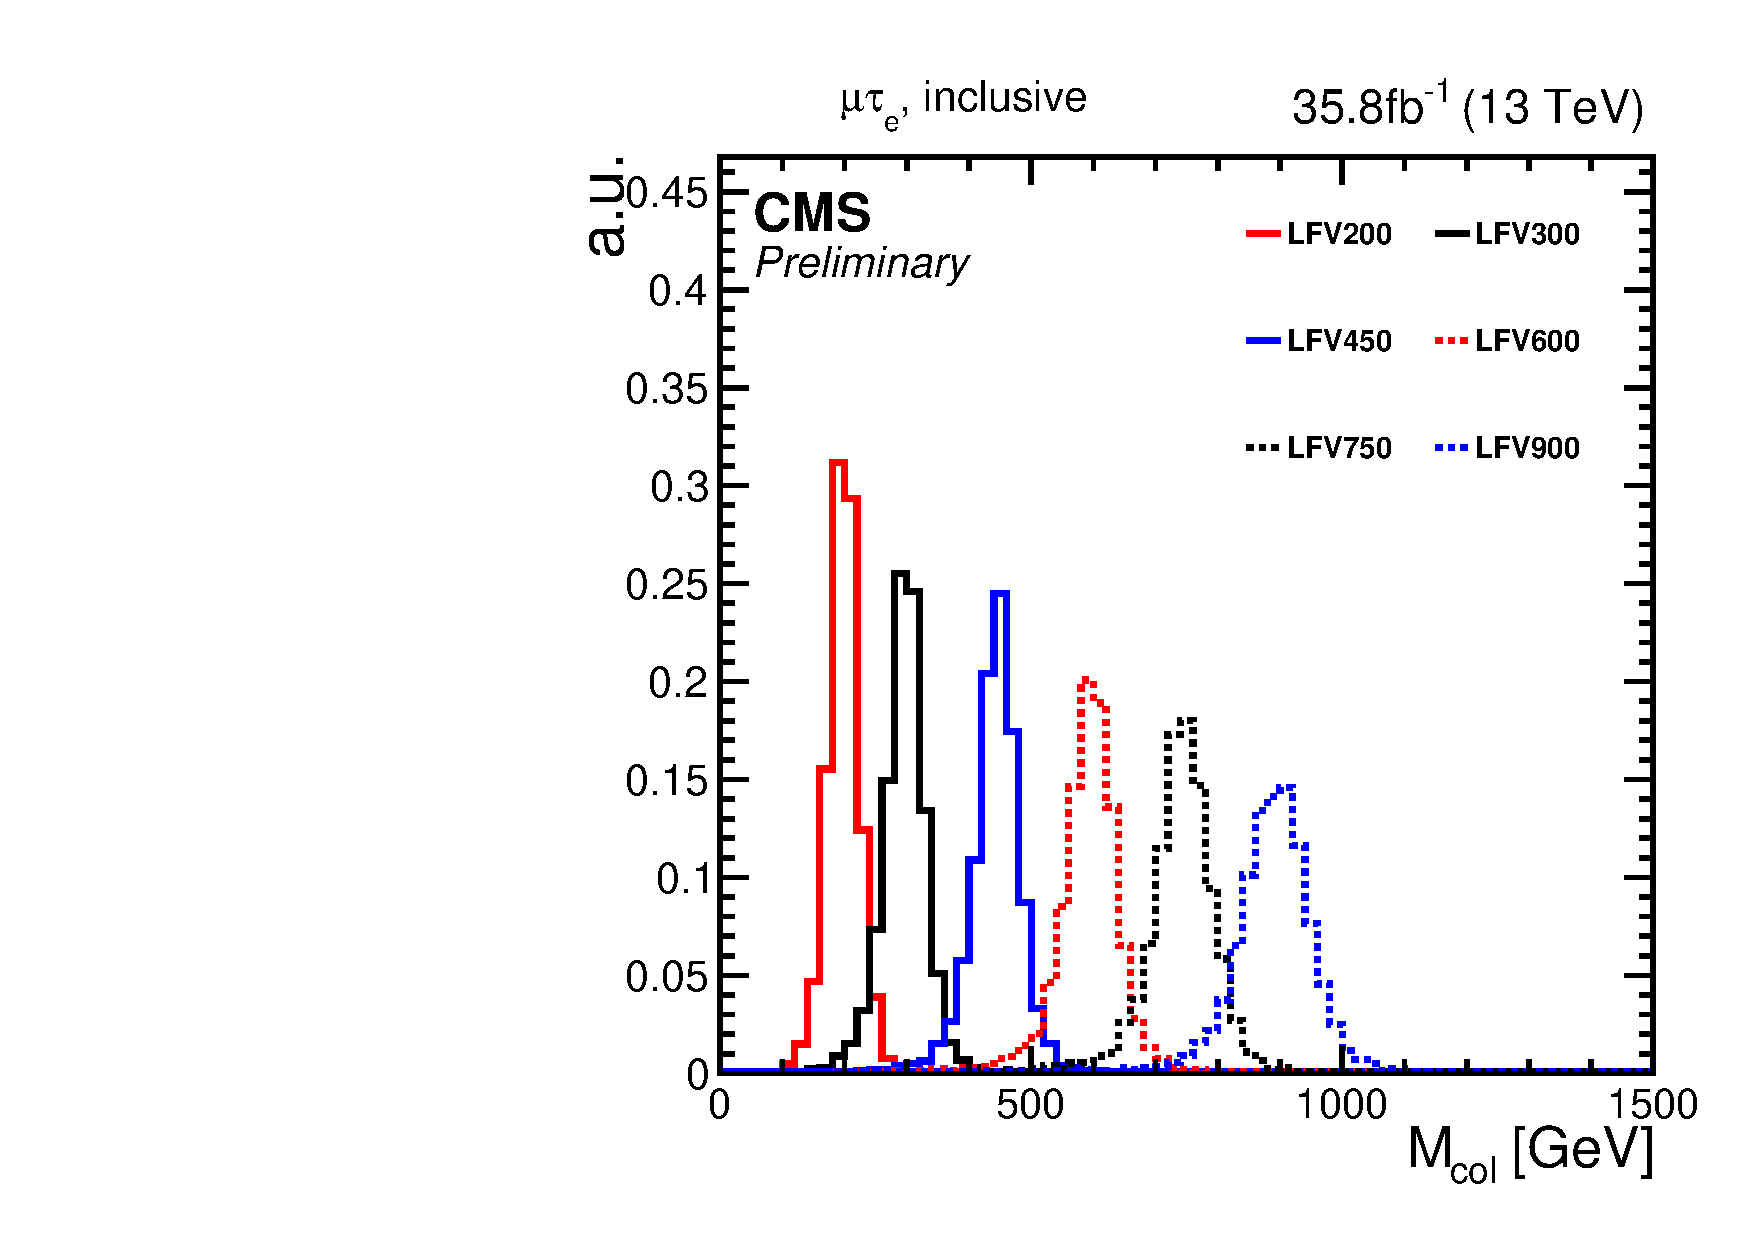
\includegraphics[width=0.5\textwidth]{plots_and_figures/chapter5/HM_signals_only_colmass.pdf}\\
     \caption{Illustration of simulated signal mass peaks for \Hmue analysis for different H boson masses.}
     \label{fig:sig_peaks}
\end{figure*}

The most dominant backgrounds for \Hmue consists of events from  \ttb and electroweak diboson production. Unlike \hmue analysis, \ztt events from Drell-Yan production form a very small background as the \ztt spectrum peaks at much lower values (around $\PZ$ boson mass) of collinear mass that the signal events coming from heavy H boson decays. The other backgrounds come from h boson decays ($\PH \to \Pgt\Pgt,\PW\PW$), $\PW\gamma^{(*)}+\text{jets}$ ,single top production, \wjets events, $Z\to\ell\ell$ $(\ell = \Pe, \Pgm)+\text{jets}$ and QCD multijet backgrounds. These backgrounds are described in more detail, along with there estimation and validation techniques in section~\ref{bg_val}.        

\subsection{\Hmue: Baseline selection and categorization}
\label{H_presel_cat}
The baseline selection for \Hmue is similar to that of \hmue with the exception of higher $\pt$ thresholds. Just like \hmue, an isolated and well-identified $\Pgm$ is thus required to be present along with an well-identified and isolated $\Pe$ of opposite sign charge. They are required to be separated by $\Delta R > 0.3$. The identification and isolation criteria have been described in sections~\ref{mu_recon},~\ref{e_recon} and ~\ref{tau_recon}. All events are required to pass a single muon trigger with the threshold of 50\GeV. The trigger selection has been described in detail in section~\ref{trigger}. The $\Pgm$ is required to have $\pt^{\Pgm} > 53$\GeV and $|\eta^{\Pgm}|<2.4$. The $\Pe$ is required to have $\pt^{\Pe} > 10$\GeV and $|\eta^{\Pe}|<2.3$. Only events with zero or one jet are considered. Jets  must have $\pt>30$\GeV, $|\eta| < 2.4 $ and satisfy the loose identification criterion described in section~\ref{jet_recon} to be considered. As only GGF production mode is considered for the \Hmue analysis, events with more than one jet make negligent contribution and are rejected. All other other criteria are same as the \hmue analysis. The entire set of baseline selection criteria for \Hmue has been summarized in table~\ref{tab:H125_base_sel}.

\begin{table*}[htpb]
 \begin{center}
 \caption{Baseline selection criteria for \Hmue analysis.}
  \begin{tabular}{c|c|c} \hline
    Variable    &  $\Pgm$  & $\Pe$ \\ \hline
    $\pt $       & $>53$\GeV &  $>10$\GeV                                           \\
    $|\eta| $       & $<2.4 $ &  $<2.3$                                           \\
    $I_{\text{rel}}$  & $<0.15$ &  $<0.1$                                           \\
    \multicolumn{3}{c}{Cleaning requirements} \\\hline
    \multicolumn{3}{c}{ $\Delta R(\Pgm,\Pe) > 0.3$} \\
    \multicolumn{3}{c}{No additional $\Pgm$, $\Pe$ or $\Pgt_{had}$} \\
    \multicolumn{3}{c}{No b-tagged jets with $\pt>30$\GeV} \\
    \multicolumn{3}{c}{No jets with $\Delta R(\Pgm,jet)<0.4$ and $\pt>30$\GeV} \\
    \multicolumn{3}{c}{No jets with $\Delta R(\Pe,jet)<0.4$ and $\pt>30$\GeV }\\
    \hline
  \end{tabular}
  \label{tab:H125_base_sel}
  \end{center}
\end{table*}

The events are then divided into  categories, with motivations similar to the \hmue analysis (see section~\ref{h125_presel_cat}), on the basis of number of jets present in the event. The two categories for \Hmue are:
\begin{itemize}%[itemsep=5pt]
\item \textbf{0-jet category}: These are events that do not have any jet. This category enhances the gluon-gluon fusion (GGF) contribution.
\item \textbf{1-jet category}: Events that have 1 jet are put in this category. This category enhances the GGF production with initial state radiation (ISR).
\end{itemize}

The distributions of several kinematic variables after the baseline selection and categorization are shown in Figs.~\ref{fig:Hmutaue_presel1} and ~\ref{fig:Hmutaue_presel2}.

\begin{figure*}[htbp]
     \centering
     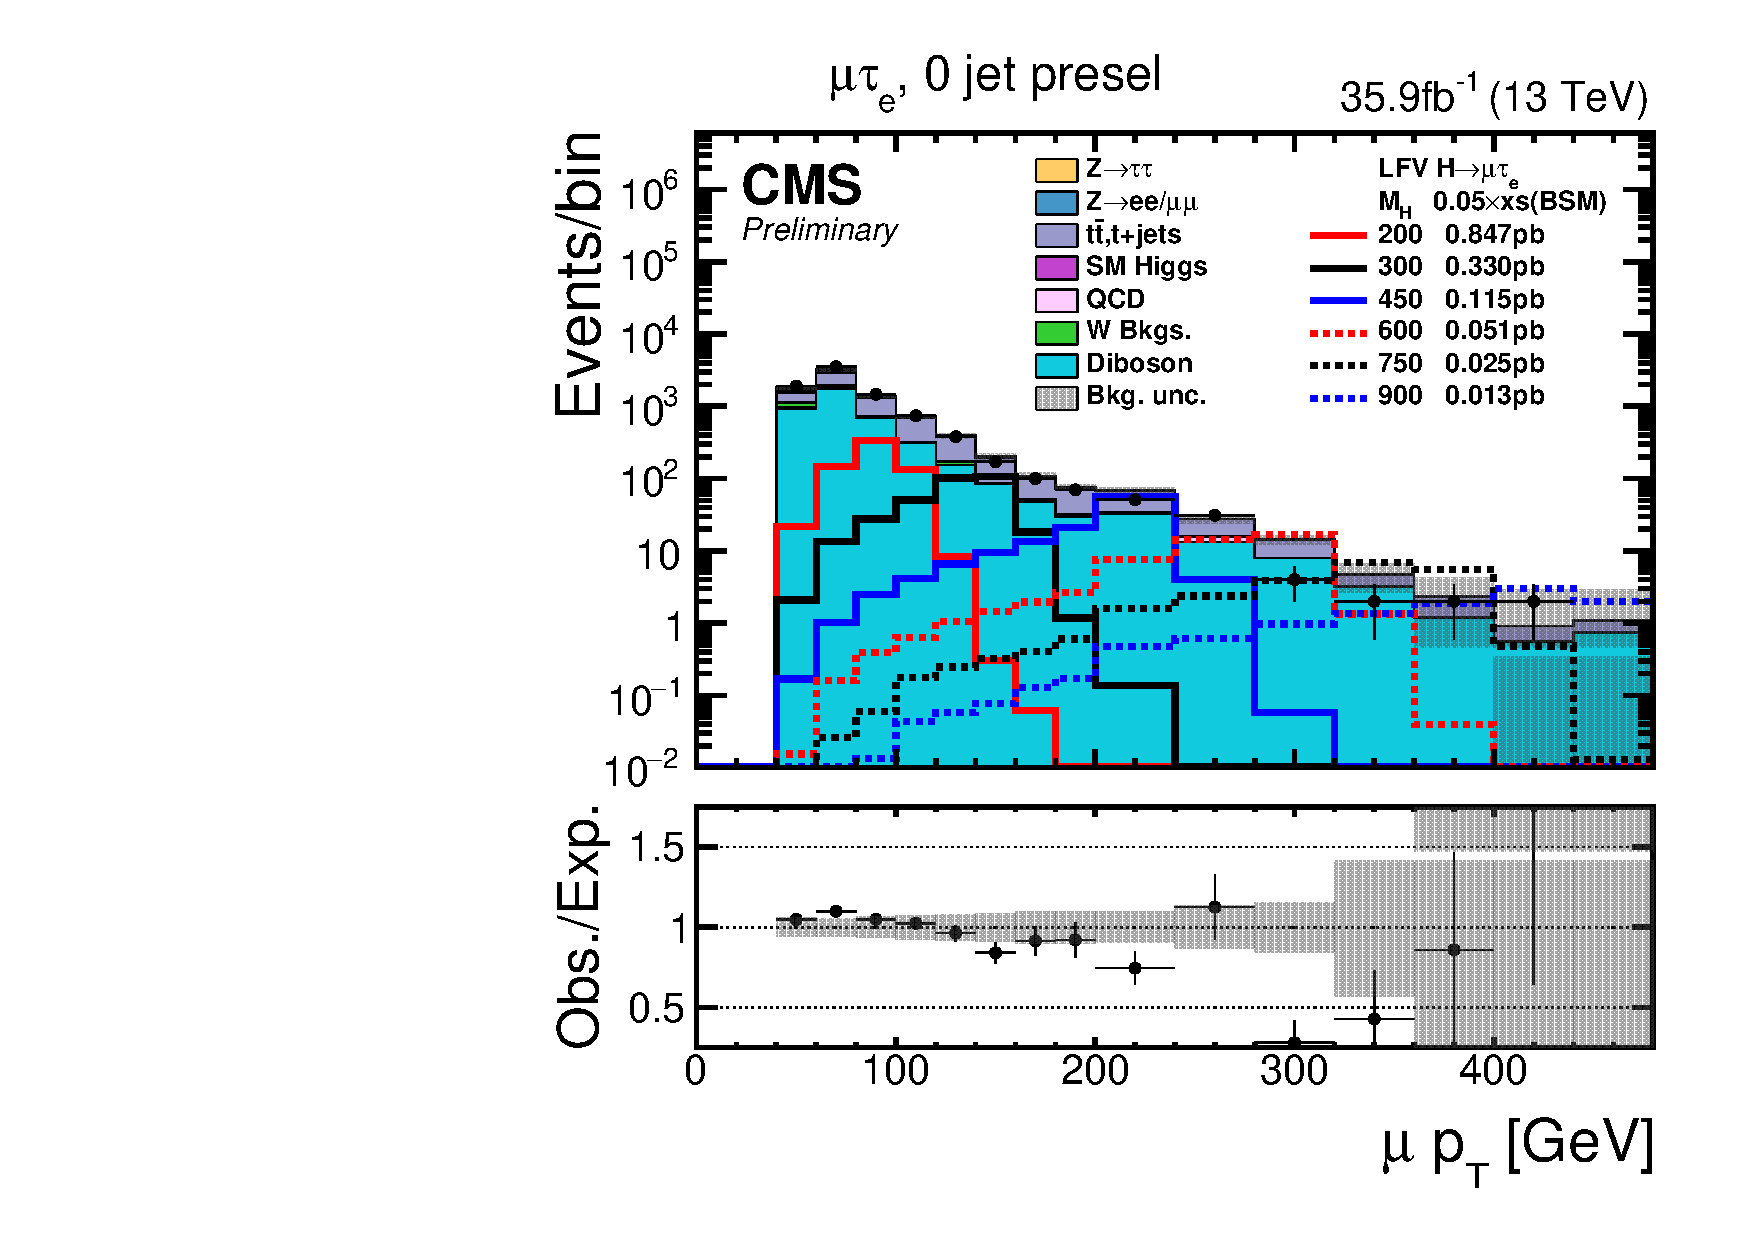
\includegraphics[width=0.48\textwidth]{plots_and_figures/chapter5/preselection_HM/log_mutaue_0jet_presel_mPt.pdf}
     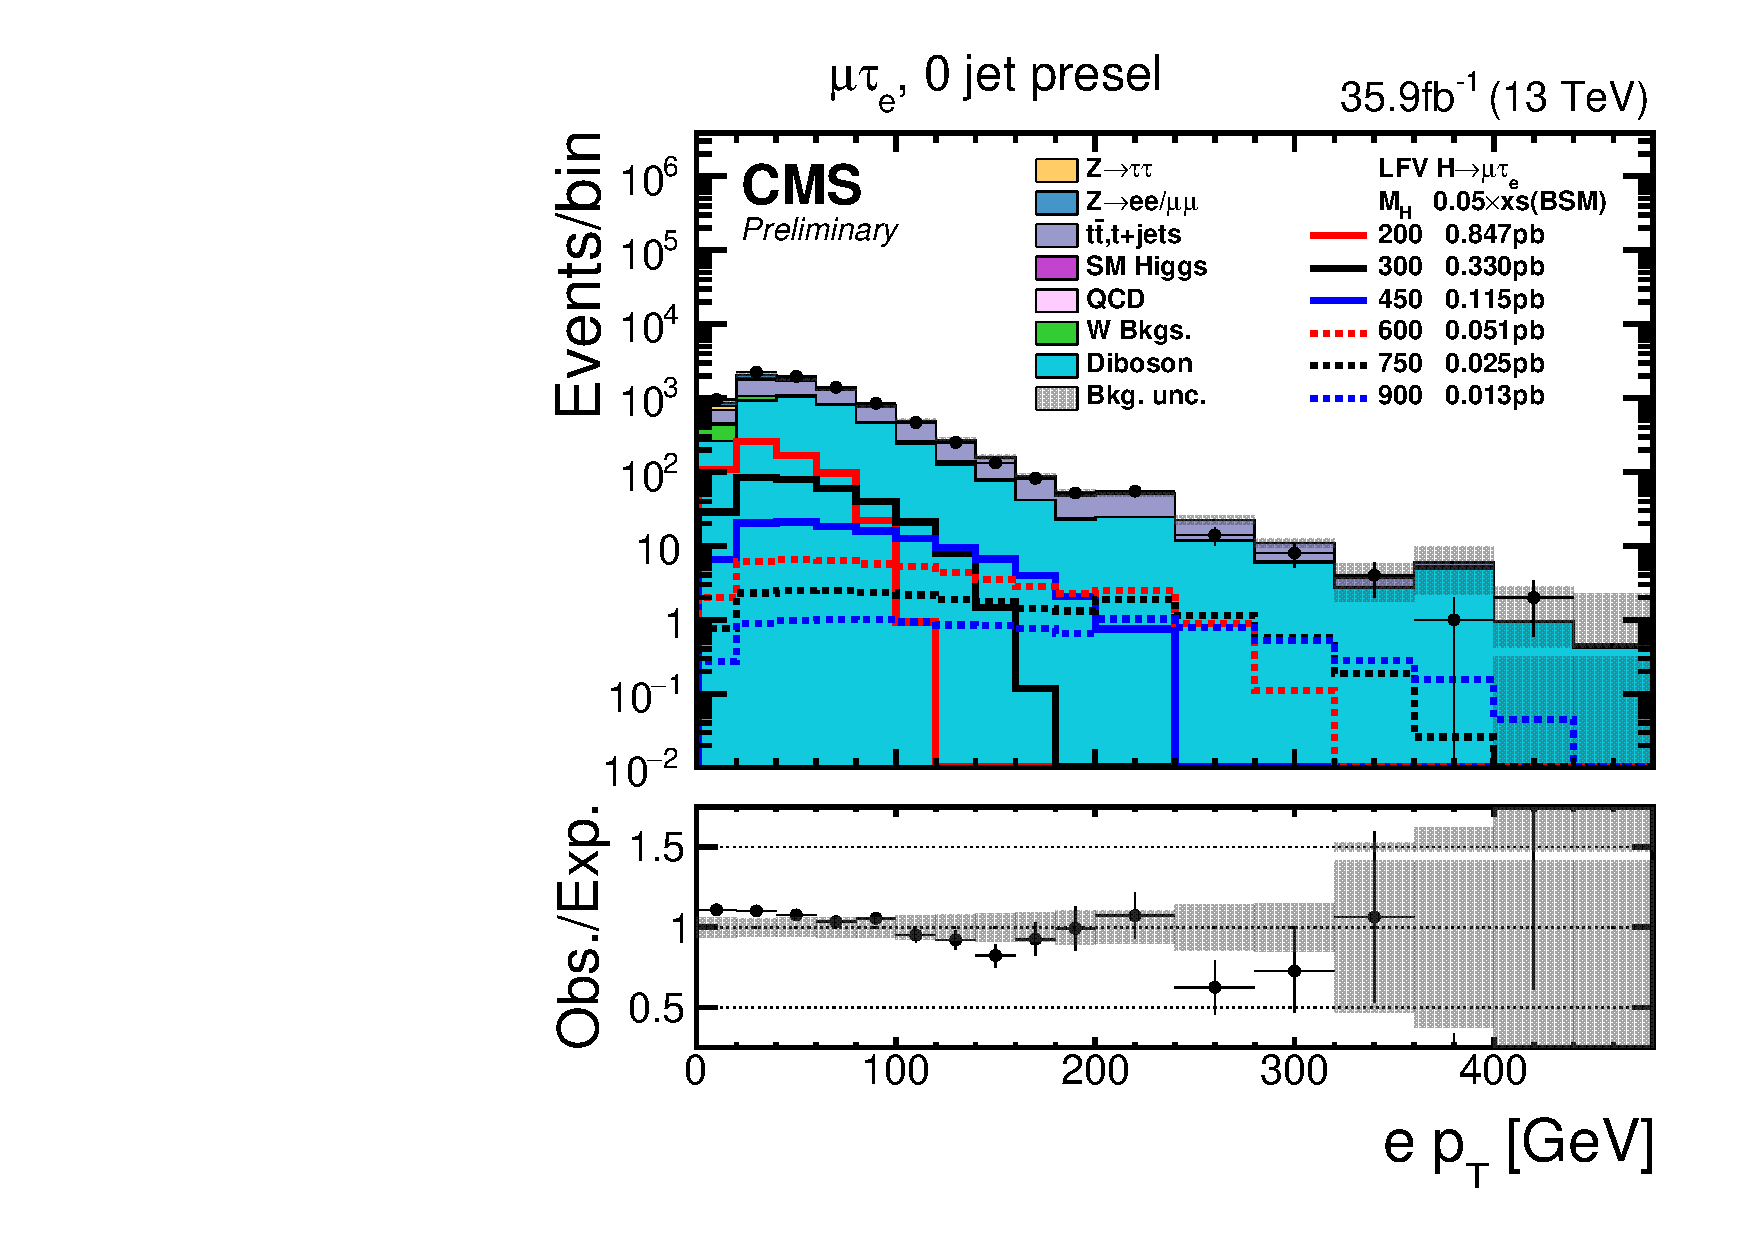
\includegraphics[width=0.48\textwidth]{plots_and_figures/chapter5/preselection_HM/log_mutaue_0jet_presel_ePt.pdf}\\
     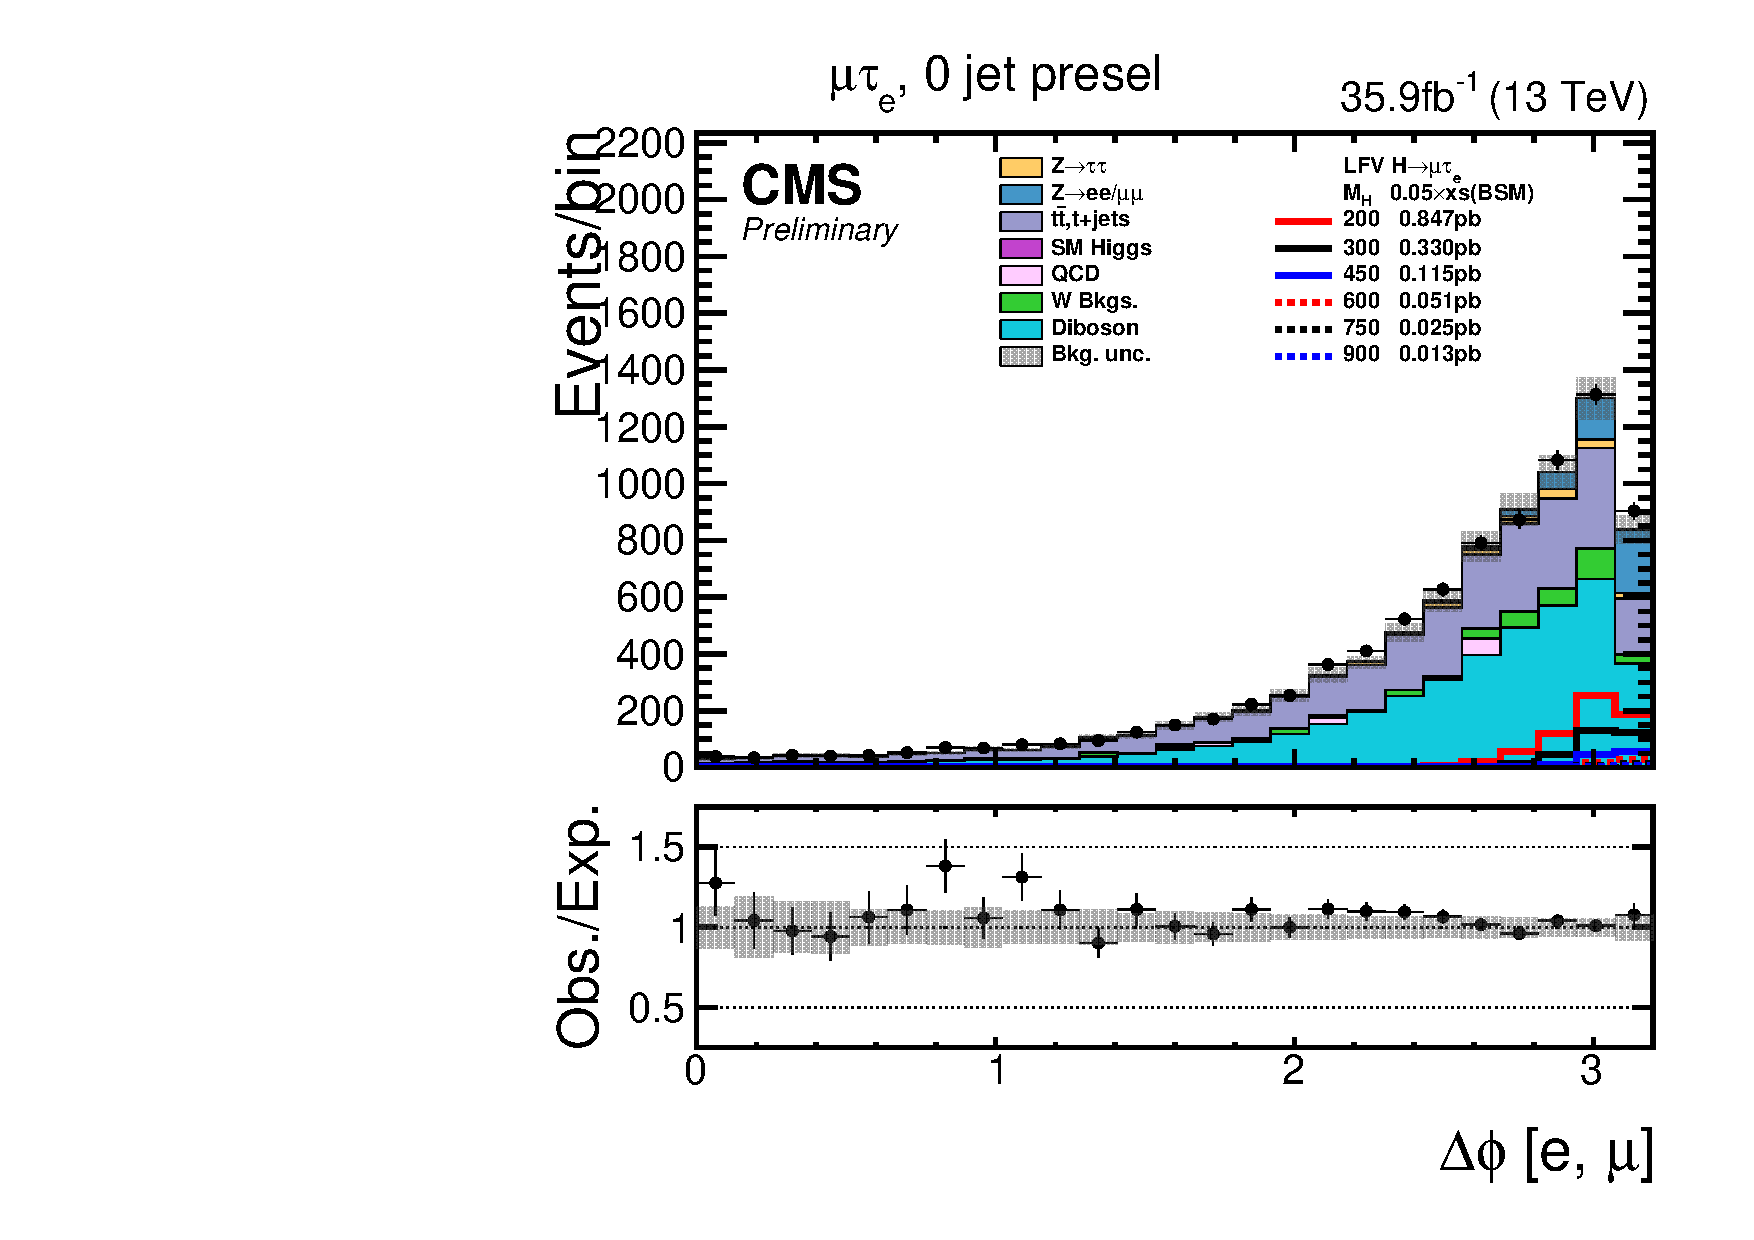
\includegraphics[width=0.48\textwidth]{plots_and_figures/chapter5/preselection_HM/mutaue_0jet_presel_dphiemu.pdf}
     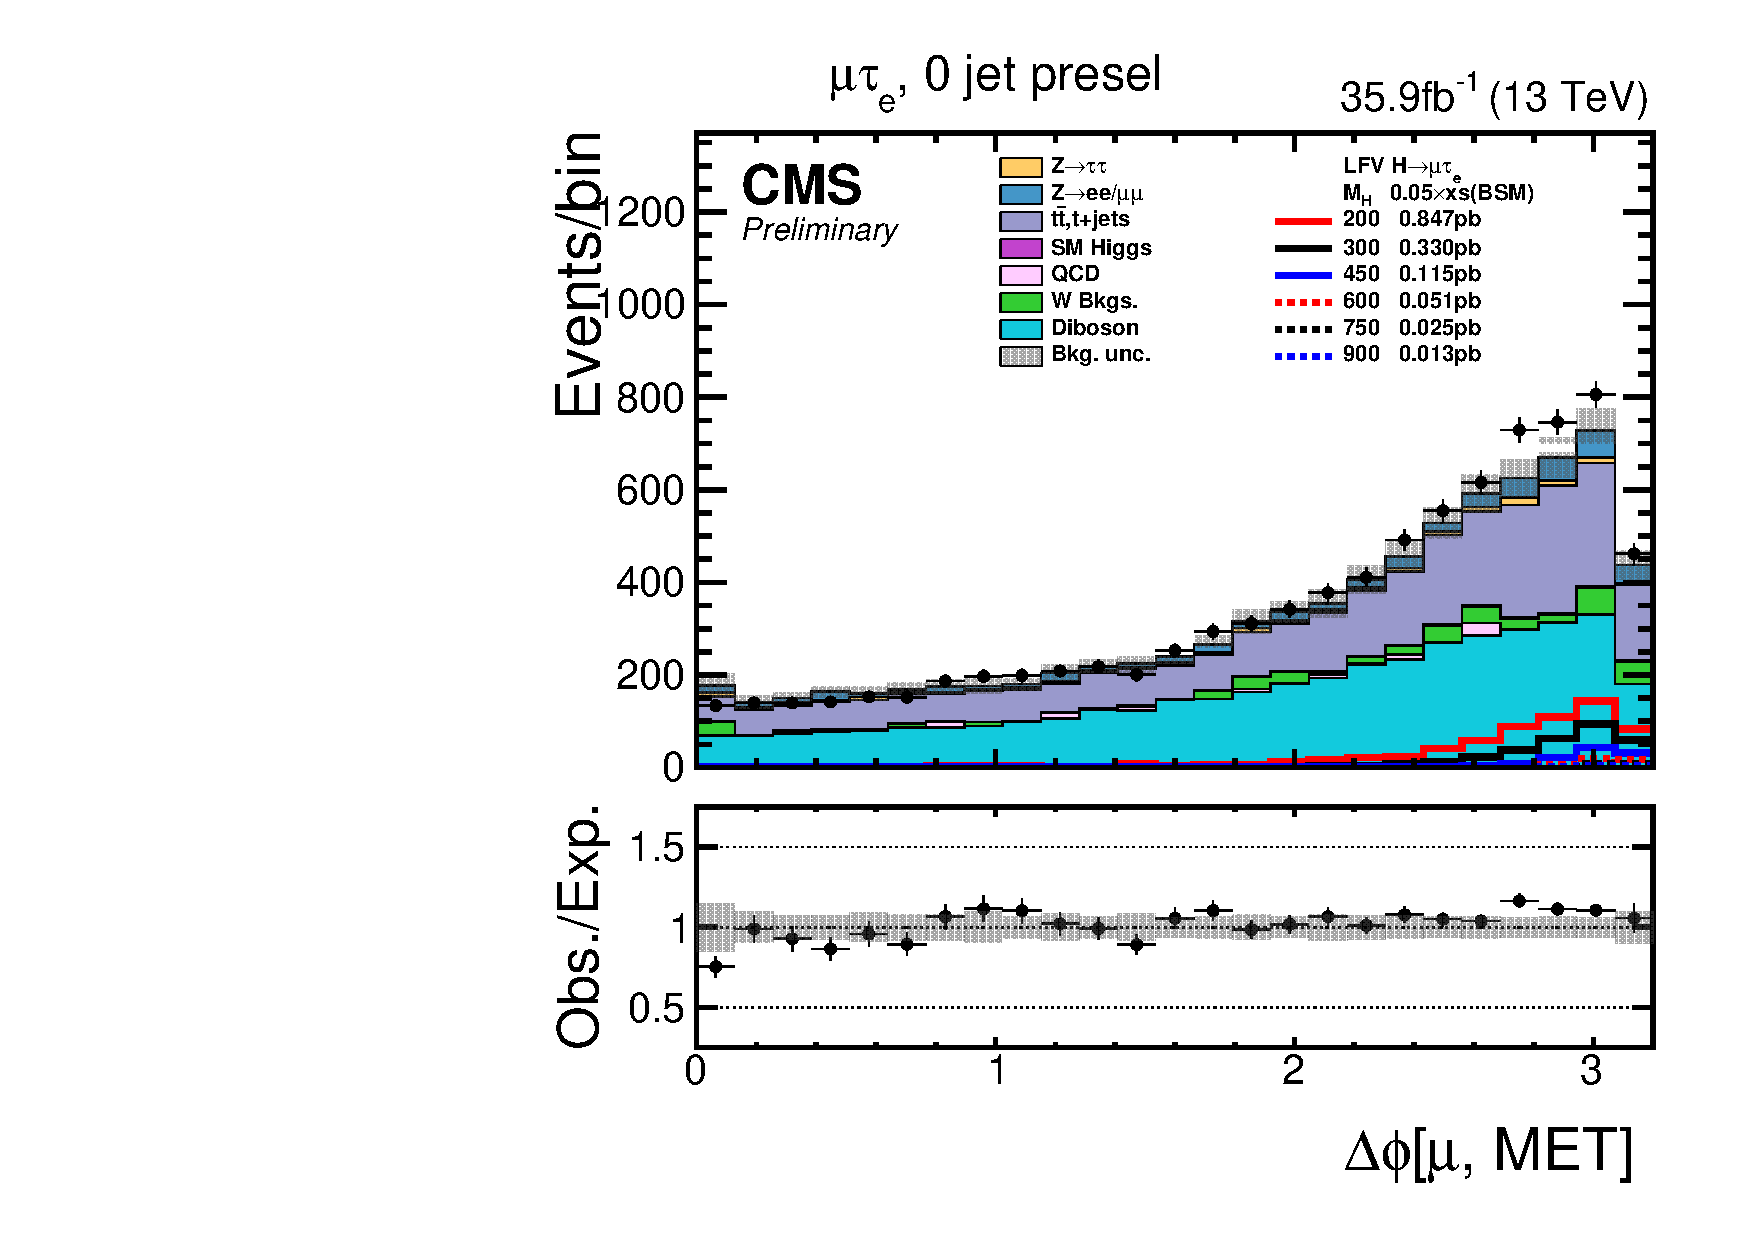
\includegraphics[width=0.48\textwidth]{plots_and_figures/chapter5/preselection_HM/mutaue_0jet_presel_dphiMuMet.pdf}\\
     \caption{Distributions of kinematic variables after baseline selction for 0-jet category of \Hmue analysis.}
     \label{fig:Hmutaue_presel1}
\end{figure*}

\begin{figure*}[htbp]
     \centering
     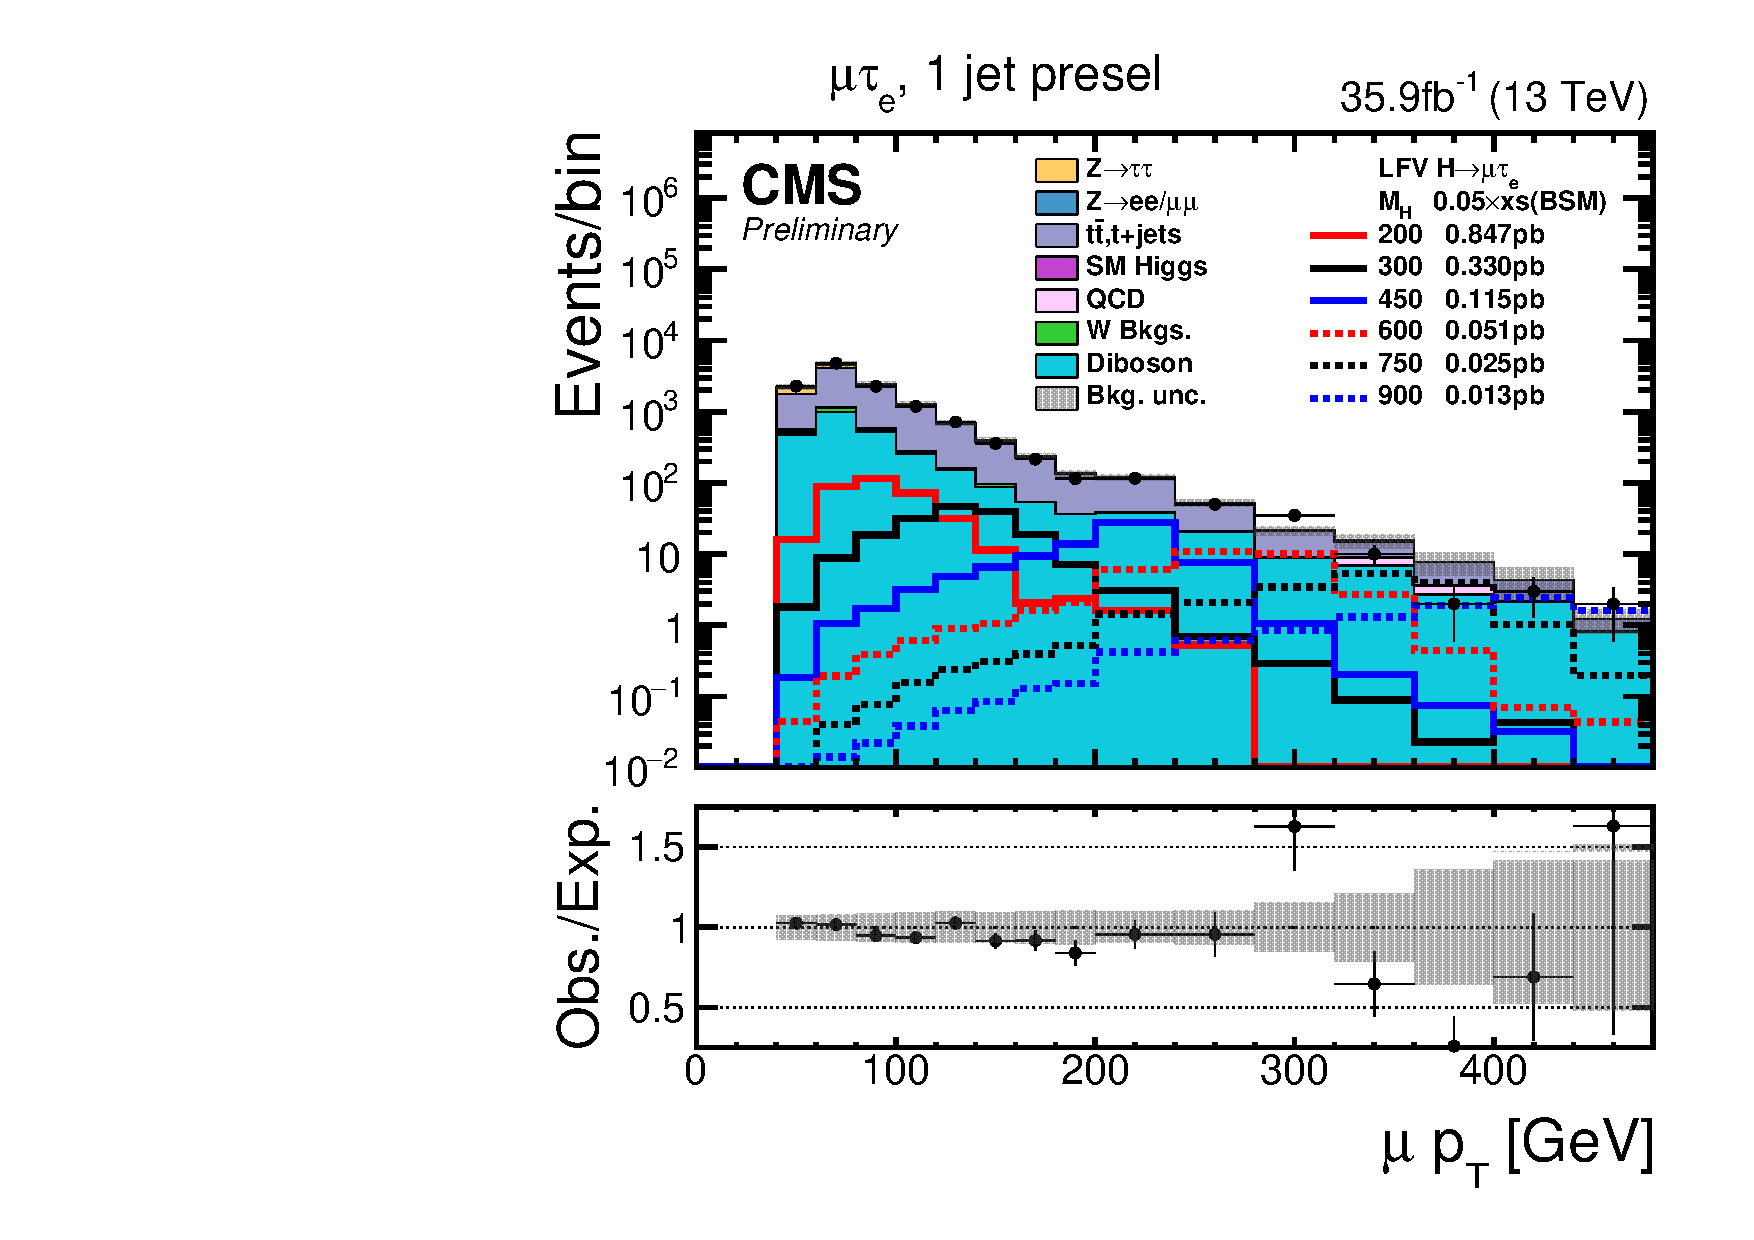
\includegraphics[width=0.48\textwidth]{plots_and_figures/chapter5/preselection_HM/log_mutaue_1jet_presel_mPt.pdf}
     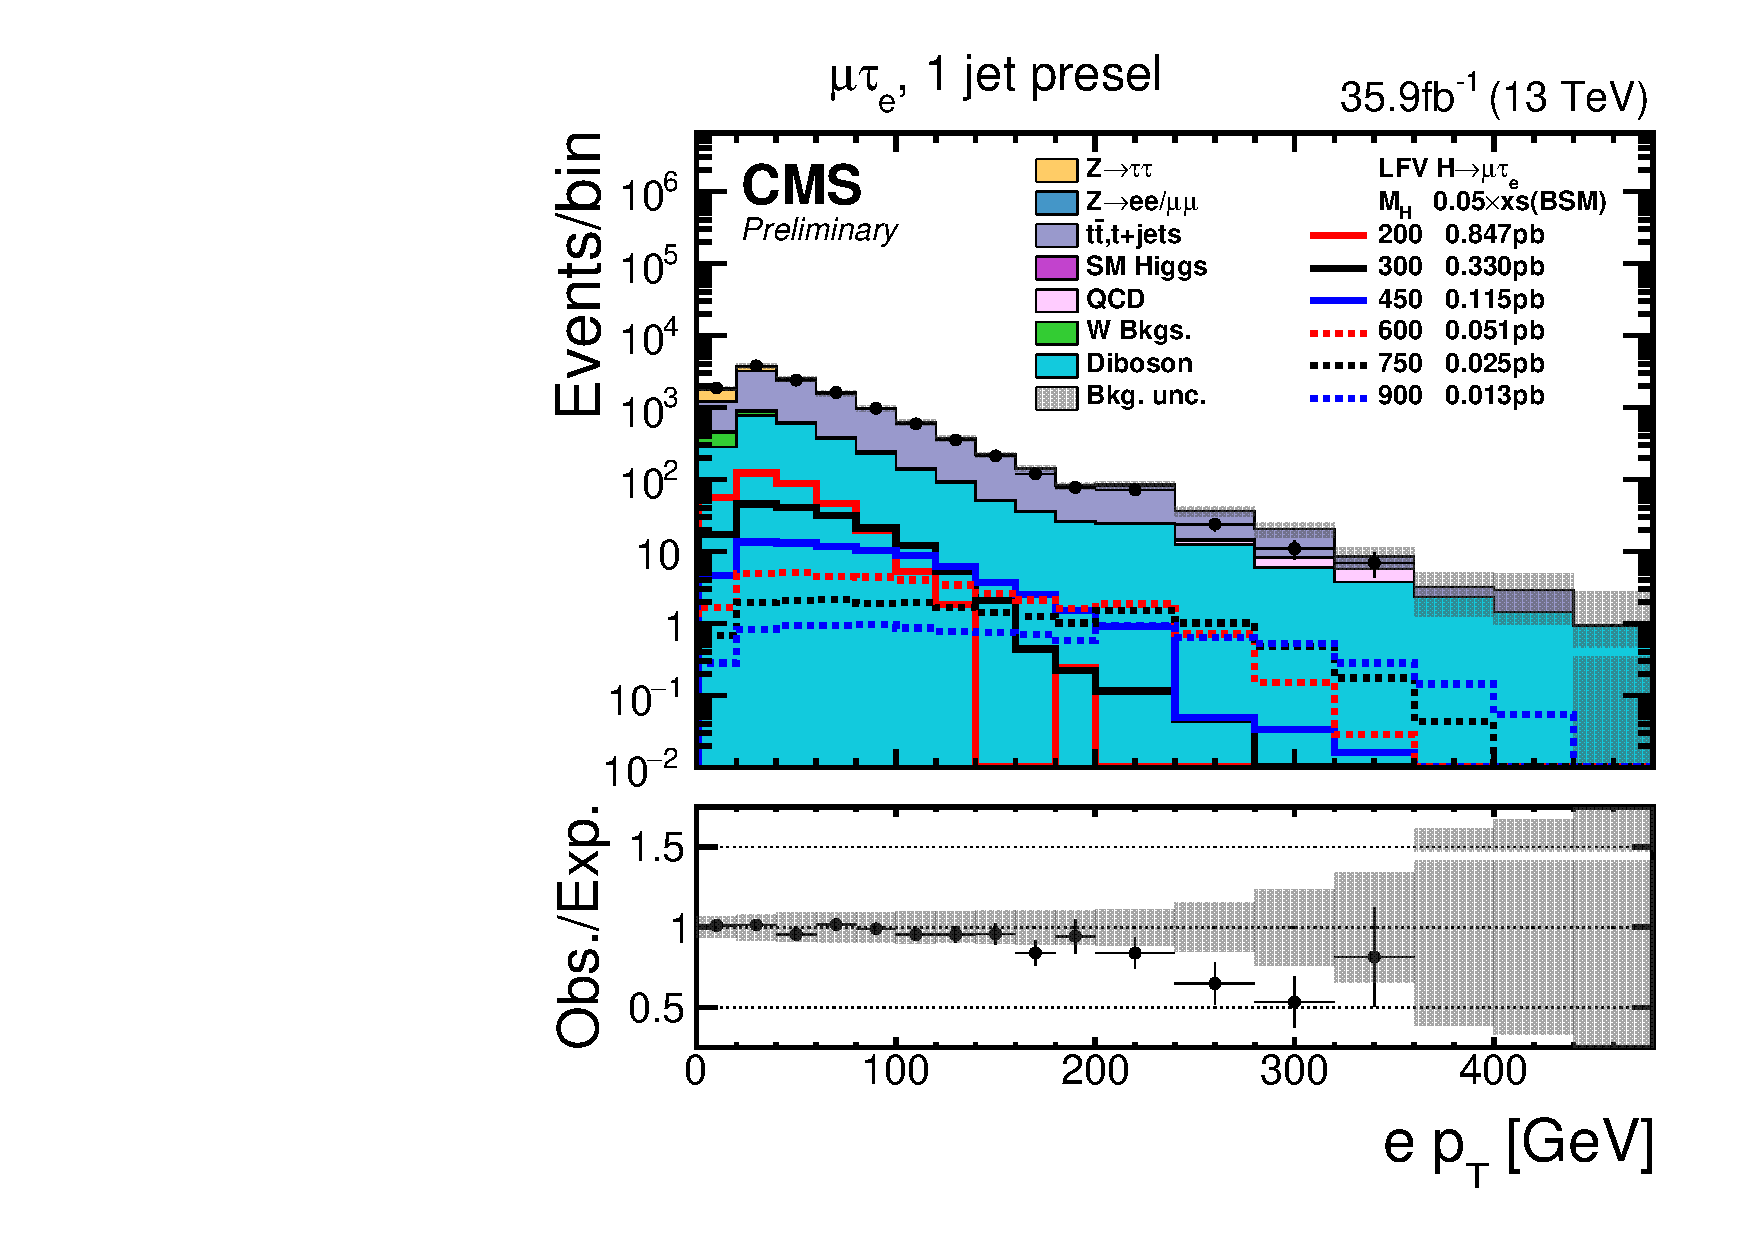
\includegraphics[width=0.48\textwidth]{plots_and_figures/chapter5/preselection_HM/log_mutaue_1jet_presel_ePt.pdf}\\
     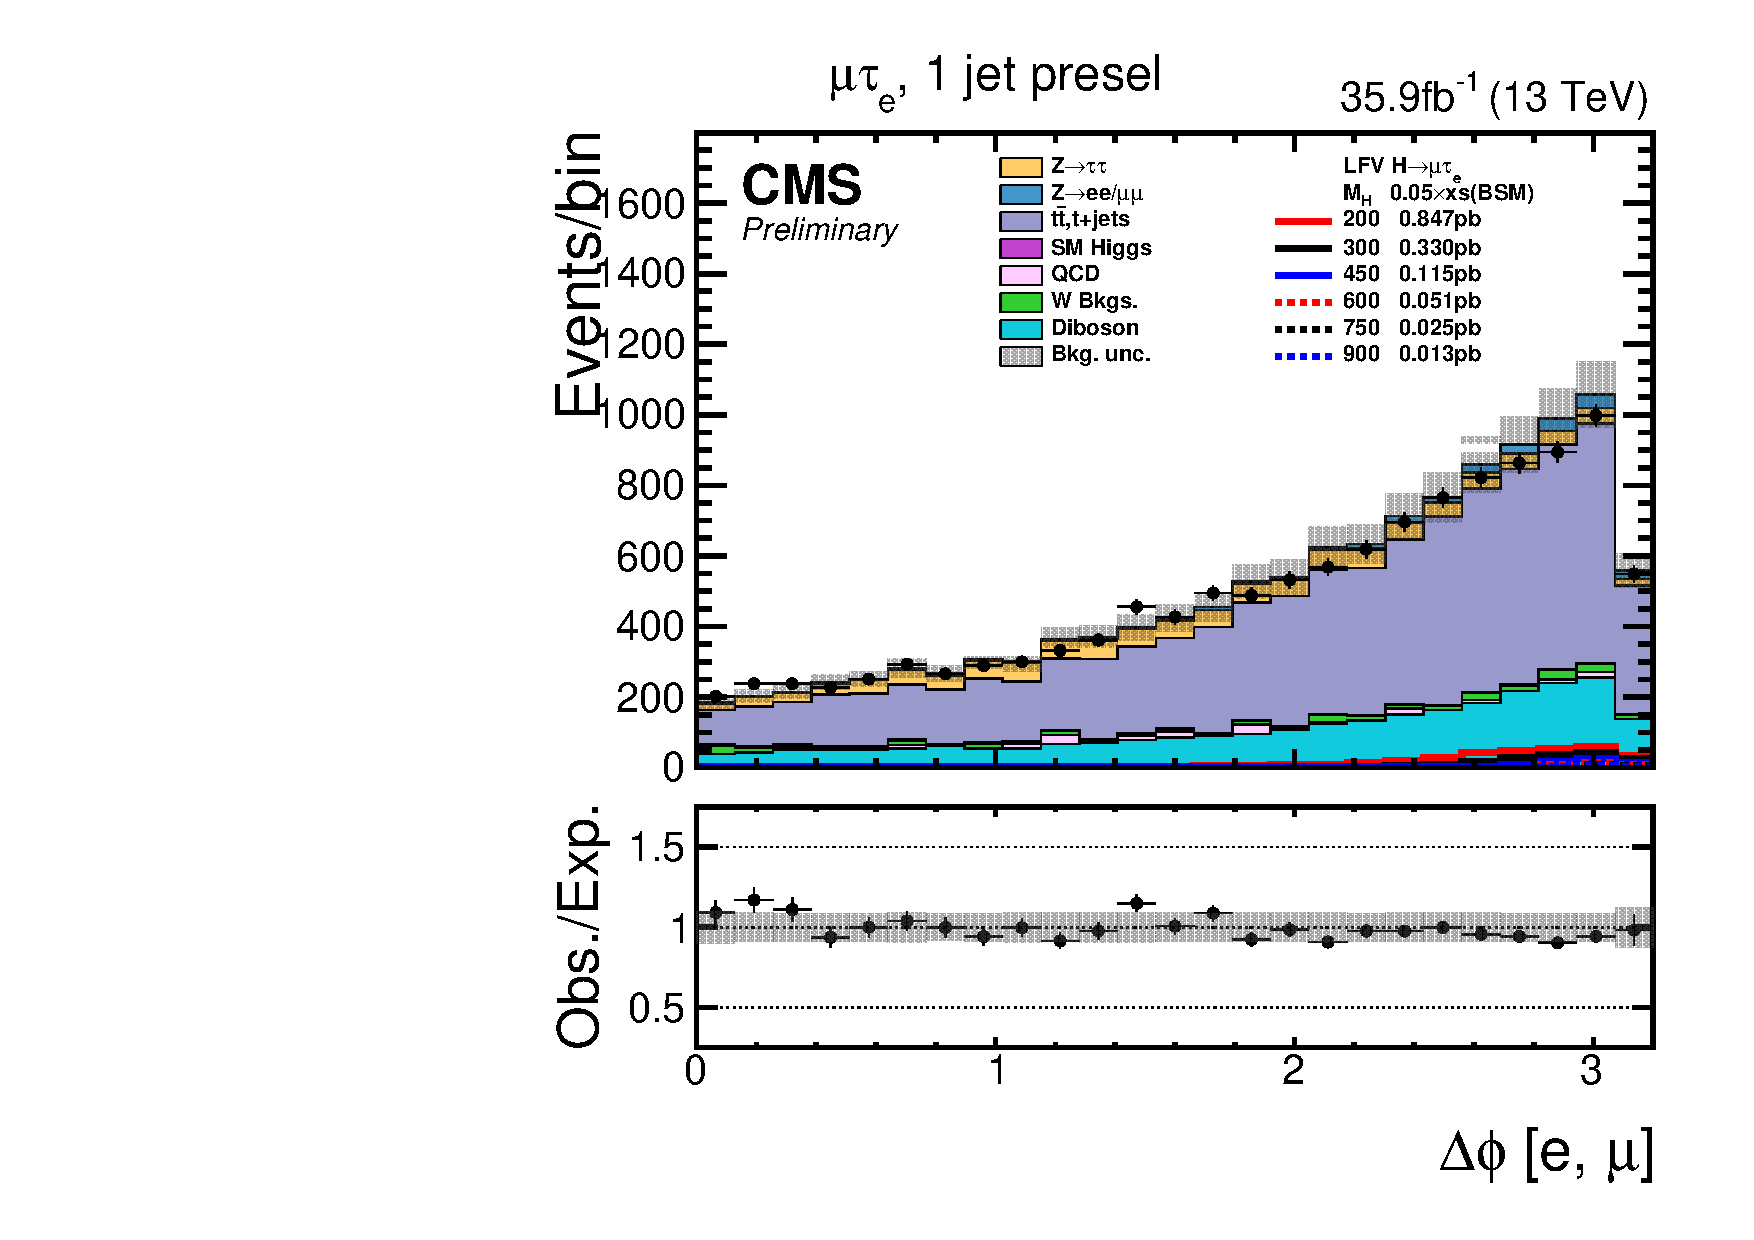
\includegraphics[width=0.48\textwidth]{plots_and_figures/chapter5/preselection_HM/mutaue_1jet_presel_dphiemu.pdf}
     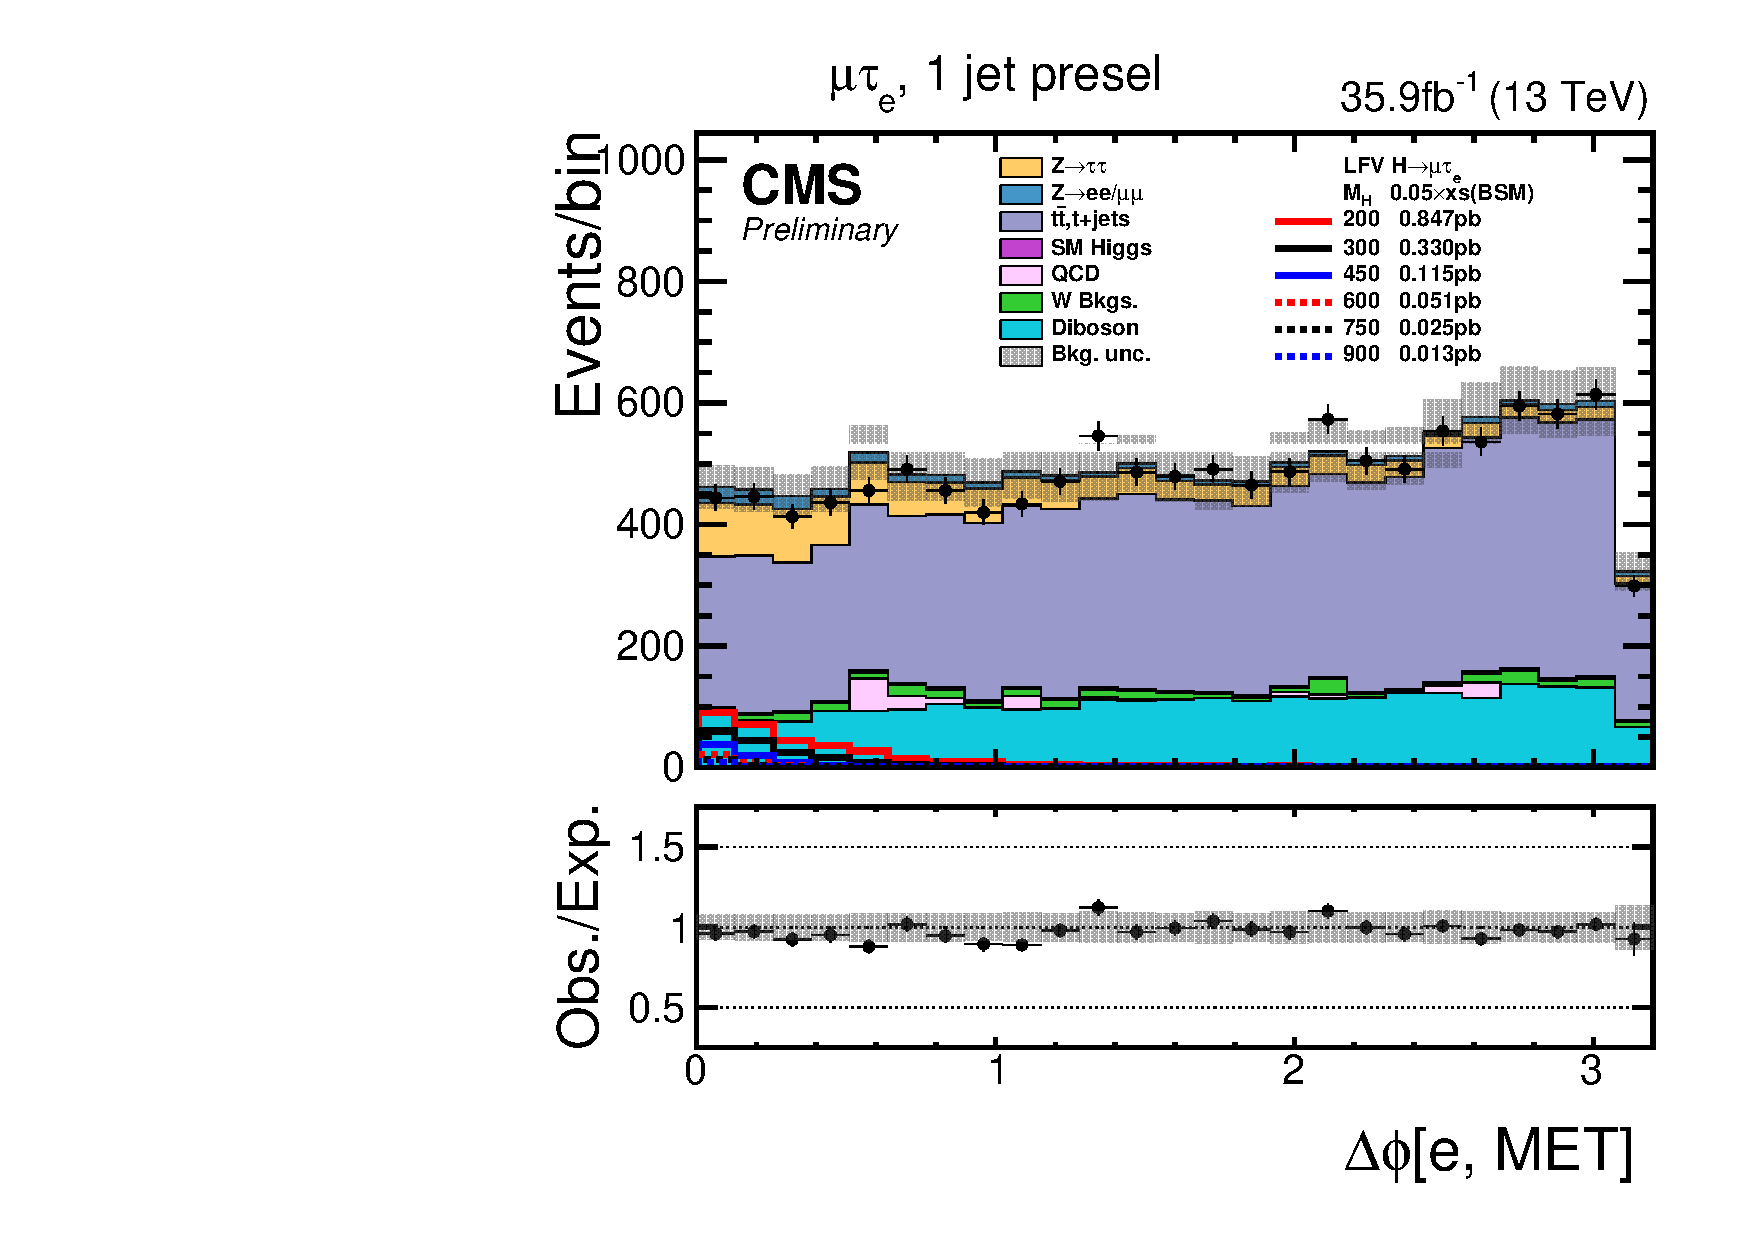
\includegraphics[width=0.48\textwidth]{plots_and_figures/chapter5/preselection_HM/mutaue_1jet_presel_dphiEMet.pdf}\\
     \caption{Distributions of kinematic variables after baseline selction for 1-jet category of \Hmue analysis.}
     \label{fig:Hmutaue_presel2}
\end{figure*}


\subsection{\Hmue: mcol fit selection}
\label{H125_cb_sel}
 Just like the \mcol fit method in \hmue, the selection is performed by placing kinematic cuts on several variables to enhance the signal-to-background ratio. The variables considered are: $\dphiemu$, $\dphiemet$, $\dphimumet$, $M_T(\Pgm)$ and $M_T(\Pe)$. In addition, the $\pt$ of the $\Pgm$ and $\Pe$ are also considered. Since we are looking for a decay in an extended mass range (200-900 GeV) in \Hmue, and not in a particular region like the \hmue analysis, the potential effect of background  mimicking the signal, in particular due to higher $\pt$ thresholds of the leptons, is not apparent. The motivations for using these variables remain much the same like the \hmue analysis owing to similarities in topology. They are motivated by the facts that the only source of MET is the $\Pgt$, and the  $\Pgt$ being lighter than the H, its visible products are closely aligned, and the $\pt$ spectrum of the prompt lepton ($\Pgm$) is hard.

The procedure for optimization of the thresholds of for these variables is exactly the same as described in section~\ref{h125_cb_sel}. Further to get better sensitivity in the entire mass range from 200 to 900 GeV, two separate sets of thresholds are optimized, for each category. One set is optimized to provide better sensitivity in the 200-450 GeV mass range. The simulated signal for the H mass of 200 GeV is used when calculating expected limits during the optimization procedure for this mass range. The other set is optimized to provide better sensitivity in 450-900 GeV mass range. The simulated signal for H mass of 450 GeV is used when calculating expected limits during the optimization procedure for this mass range. A few illustrations of the optimization procedure are shown in Fig.~\ref{fig:Hmue_limit_opt}. The final set of thresholds arrived at in this manner, for both mass ranges and both categories of the \Hmue \mcol fit analysis, are listed in Table.~\ref{tab:H125_sel_cuts}. The \mcol distributions after requiring these selections is used in a max-likelihood fit to extract results, as discussed in section~\ref{sig_ext}.


 \begin{figure}[htbp]
     \centering
     \subfigure[Low mass range 0 jet $\Delta\phi(\Pe, \ptvecmiss)$]{ 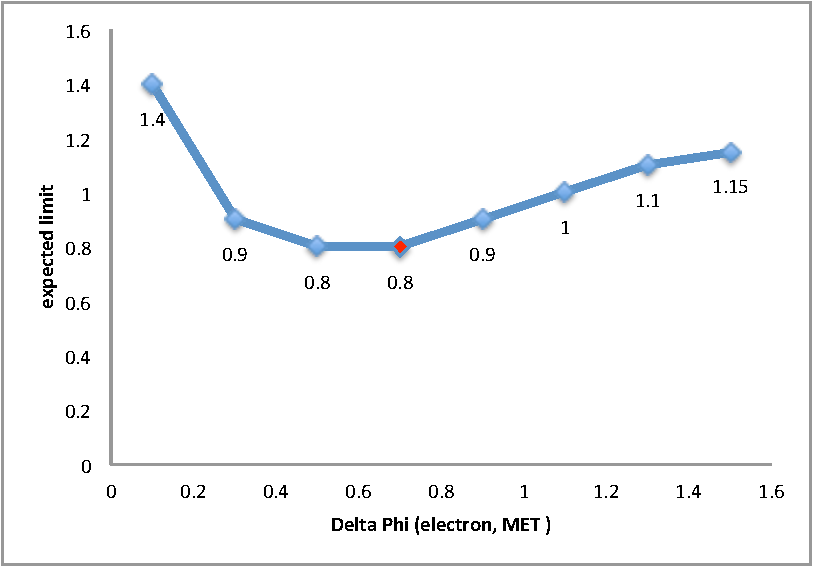
\includegraphics[width=0.375\textwidth]{plots_and_figures/chapter5/limit_opt/200_0jet_dphiemet.pdf}}
     \subfigure[Low mass range 1 jet $\Delta\phi(\Pe, \ptvecmiss)$]{ 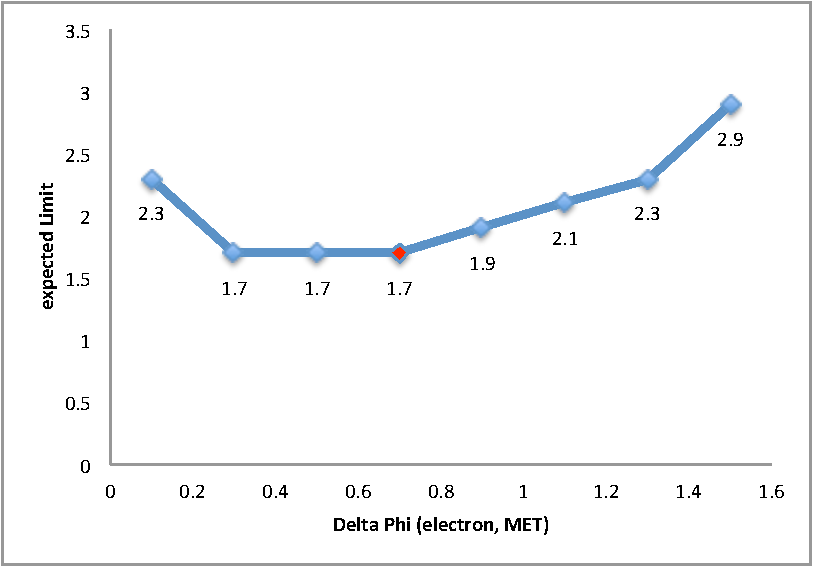
\includegraphics[width=0.375\textwidth]{plots_and_figures/chapter5/limit_opt/200_1jet_dphiemet.pdf}}\\
     \subfigure[Low mass range 0 jet $\Delta\phi(\Pe, \Pgm)$]{ 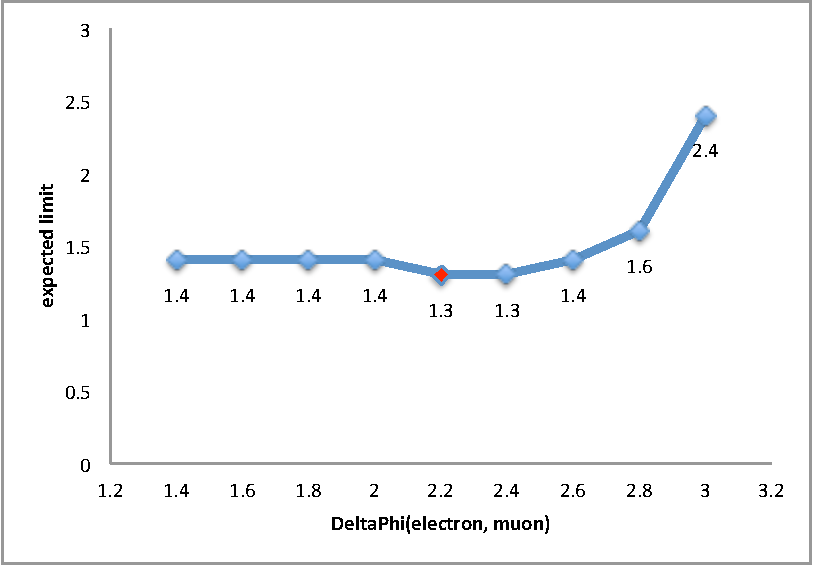
\includegraphics[width=0.375\textwidth]{plots_and_figures/chapter5/limit_opt/200_0jet_dphiemu.pdf}}
     \subfigure[Low mass range 0 jet $\pt^{\Pe}$]{ 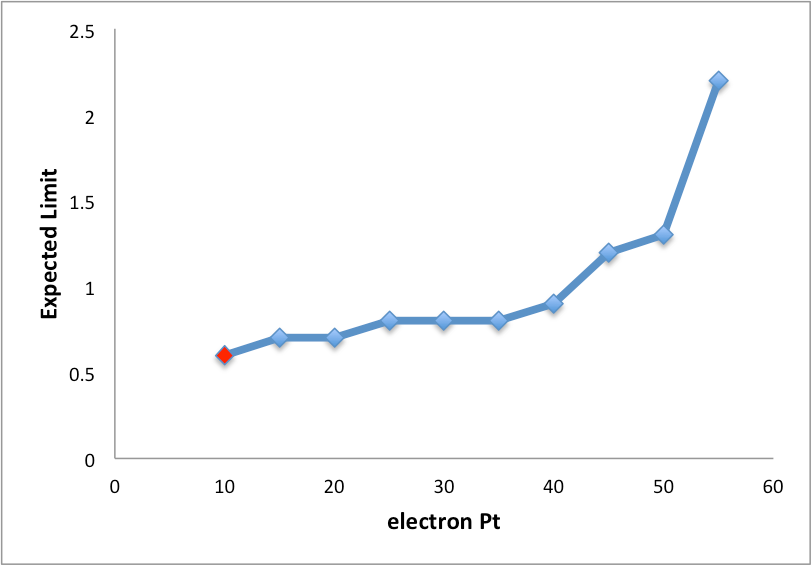
\includegraphics[width=0.375\textwidth]{plots_and_figures/chapter5/limit_opt/200_0jet_ept.pdf}}\\
     \subfigure[High mass range 1 jet $\pt^{\Pgm}$]{ 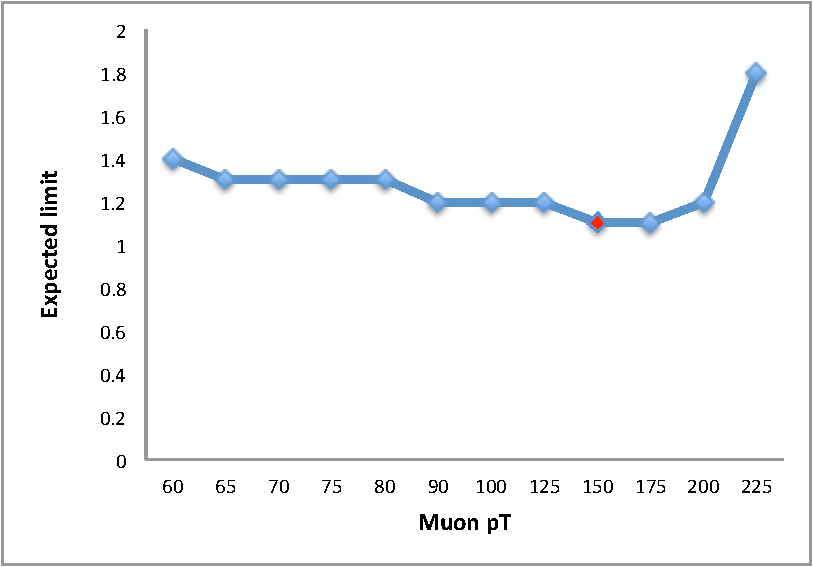
\includegraphics[width=0.375\textwidth]{plots_and_figures/chapter5/limit_opt/450_1jet_mupt.pdf}}
     \subfigure[High mass range 0 jet $\Delta\phi(\Pe, \ptvecmiss)$]{ 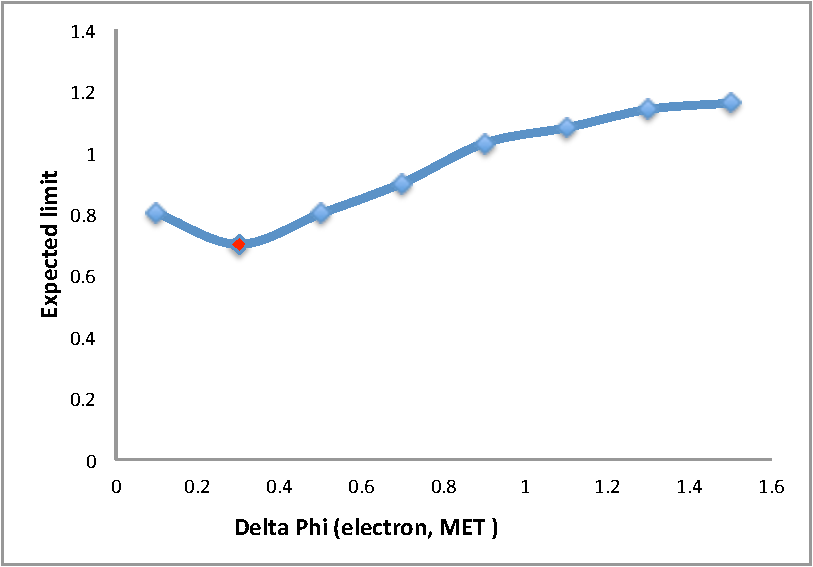
\includegraphics[width=0.375\textwidth]{plots_and_figures/chapter5/limit_opt/450_0jet_dphiemet.pdf}}\\
     \subfigure[High mass range 1 jet $\Delta\phi(\Pe, \ptvecmiss)$]{ 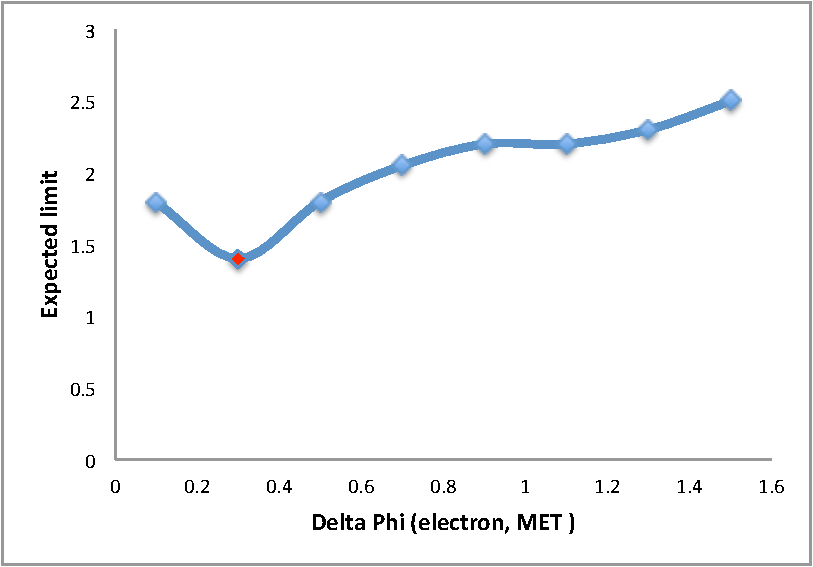
\includegraphics[width=0.375\textwidth]{plots_and_figures/chapter5/limit_opt/450_1jet_dphiemet.pdf}}
     \subfigure[High mass range 1 jet $\pt^{\Pe}$]{ 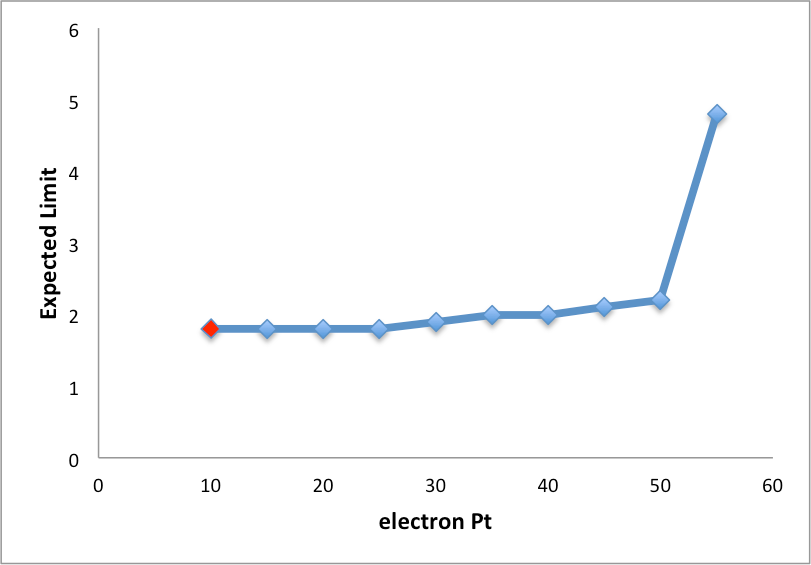
\includegraphics[width=0.375\textwidth]{plots_and_figures/chapter5/limit_opt/450_1jet_ept.pdf}}\\
     \caption{Examples of cut optimisation for the $\Hmue$ analysis}
     \label{fig:Hmue_limit_opt}
\end{figure}

 \begin{table}[hbtp]
  \begin{center}
  \caption{Final selection criteria in each category  of the $\Hmue$ analysis.}
  \begin{tabular}{c|c|c}
  \hline
  & Low mass range & High mass range\\ \hline
  \multirow{3}{*}{0-jet}
  & $\pt^{\Pgm}>60$\GeV, $\pt^{\Pe}>10$\GeV &  $\pt^{\Pgm}>150$\GeV, $\pt^{\Pe}>10$\GeV\\
  & $\Delta\phi(\Pe, \ptvecmiss)<0.7$ & $\Delta\phi(\Pe, \ptvecmiss)<0.3$ \\
  & $\Delta\phi(\Pe, \Pgm)>2.2$ & $\Delta\phi(\Pe, \Pgm)>2.2$ \\ \hline
  \multirow{3}{*}{1-jet}
  & $\pt^{\Pgm}>60$\GeV, $\pt^{\Pe}>10$\GeV & $\pt^{\Pgm}>150$\GeV, $\pt^{\Pe}>10$\GeV\\
  & $\Delta\phi(\Pe, \ptvecmiss)<0.7$ & $\Delta\phi(\Pe, \ptvecmiss)<0.3$\\
  & $\Delta\phi(\Pe, \Pgm)>2.2$& $\Delta\phi(\Pe, \Pgm)>2.2$\\
  \hline
  \end{tabular}
   \label{tab:H125_sel_cuts}
\end{center}
\end{table}







% % uncomment the following lines,
% if using chapter-wise bibliography
%
% \bibliographystyle{ndnatbib}
% \bibliography{example}
